% Phân tích sâu bốn ván, \input trong mục "Ván đấu minh hoạ" của 04-thuc-nghiem.tex.
% Số liệu từ report/chuyen-sau/data/phan-tich-van-sau.json và kiem-tra-thay-the.json; hình, bảng do bang_van_sau.py sinh.
\subsection{Phân tích sâu bốn ván: cách làm}
\label{sec:cs-van-sau}
Bốn ván được phân tích là các ván báo cáo đã dùng: ván 13 (L7--L8) và ván 26 (L3--L8) của hai lượt đấu ở trên, ván 1202
(L2 thắng L8) và ván 2726 (L7 thắng L8) của giải tám cấp trên khai cuộc giữ riêng. Không chơi thêm ván nào; mọi nước
lấy từ log. Mỗi nước được hai trọng tài xem xét:
\begin{description}
  \item[Bộ giải thắng ép.] Mở rộng bộ giải chuỗi tứ (Thuật toán~\ref{alg:cs-vcf}) sang cả ba hở: một nước là đe doạ nếu
  sau nó, giả sử đối thủ bỏ lượt, bên công có chuỗi tứ thắng. Bên thủ được thử \emph{mọi} ô trống; ô nào không phá được
  đe doạ thì thua, các ô còn lại phải bị bác bỏ bằng đệ quy. Vì vét hết đáp trả, khi bộ giải báo ``thắng ép'' thì đó là
  chứng minh. Độ sâu là số đe doạ trước khi tới chuỗi tứ: 2 cho mọi nước, mở rộng tới 3 khi lùi từ điểm quyết định.
  \item[KataGomo.] Engine mạnh độc lập \cite{katagomo}, 1\,600 lượt thăm mỗi thế. Điểm báo cáo là điểm kỳ vọng (thắng
  cộng nửa hoà) và nước nó đề nghị. Đây là \emph{ước lượng}, không phải chứng minh; mô hình được huấn luyện trên bàn
  15$\times$15 và dùng ở 11$\times$11.
\end{description}
\textbf{Nước khoá ván} là nước đầu tiên mà từ đó bên thắng luôn có đường thắng ép đã chứng minh. Ở nước ngay trước đó,
script liệt kê các ô mà sau khi đi, đối thủ không còn đường thắng ép trong cùng độ sâu. Mỗi ô như vậy được kiểm thêm
bằng tìm kiếm sâu hơn một bậc (ba đe doạ) và bằng KataGomo (Bảng~\ref{tab:cs-vs-thay-the}). Chỉ khi còn ô vượt qua cả
hai phép kiểm (không bị bác bỏ và được engine chấm từ $20\%$) thì nước đã đi mới được gọi là \textbf{sai lầm quyết định}.
\begin{figure}[H]
  \centering
  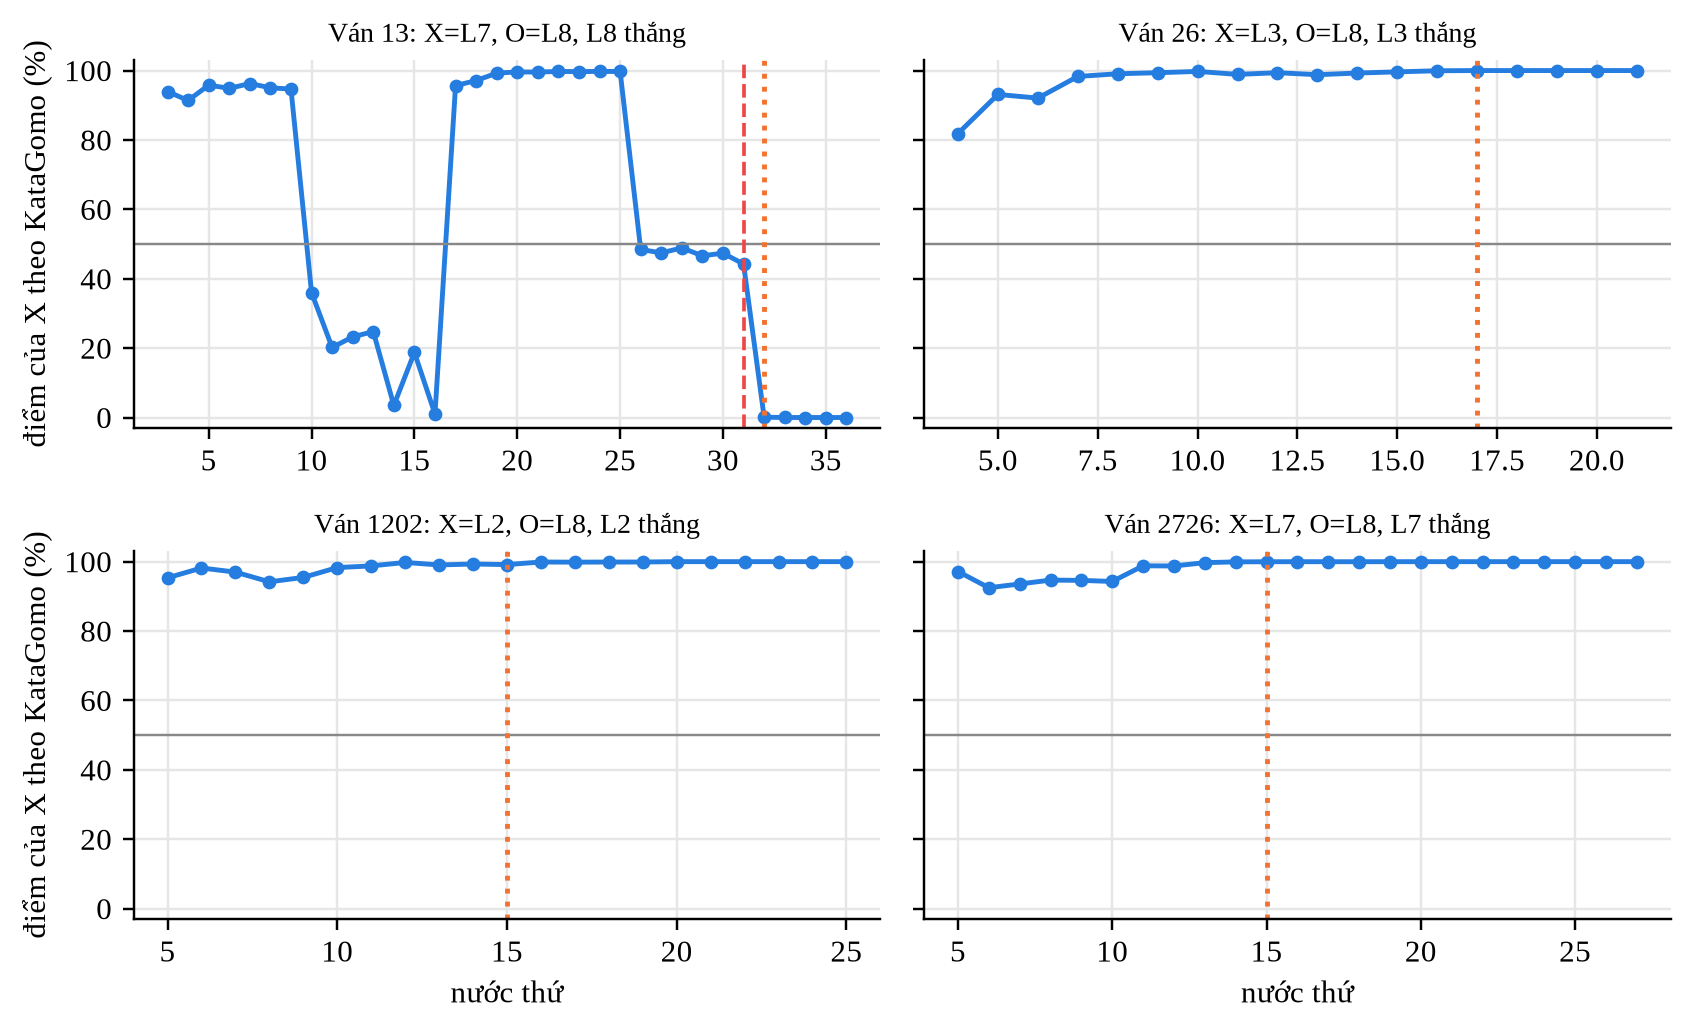
\includegraphics[width=\linewidth]{chuyen-sau/hinh/vs-ty-le-thang.png}
  \caption{Điểm của X theo KataGomo trước mỗi nước. Đường đỏ đứt: sai lầm quyết định (chỉ ván 13 có); đường cam chấm: nước khoá ván.}
  \label{fig:cs-vs-ty-le}
\end{figure}

\subsection{Ván 13: L8 thắng L7 sau khi cả hai cùng bỏ lỡ}
\label{sec:cs-vs-13}
L7 cầm X, L8 cầm O, khai cuộc F7--E4. KataGomo chấm khai cuộc này rất có lợi cho X ($94\%$ trước nước 3).
\begin{figure}[!htbp]
  \centering
  \begin{subfigure}[t]{.48\linewidth}
    \centering
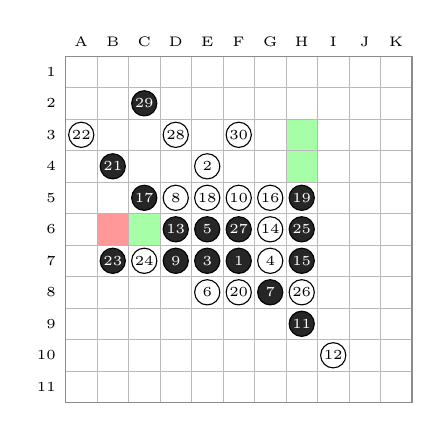
\begin{tikzpicture}[x=0.4cm, y=0.4cm]
\fill[green!35] (7,-2) rectangle (8,-3);
\fill[green!35] (7,-3) rectangle (8,-4);
\fill[green!35] (2,-5) rectangle (3,-6);
\fill[red!40] (1,-5) rectangle (2,-6);
\draw[gray!55, line width=.3pt, step=1] (0,0) grid (11,-11);
\draw[gray!90] (0,0) rectangle (11,-11);
\node[font=\tiny, anchor=south] at (0.5,0) {A};
\node[font=\tiny, anchor=south] at (1.5,0) {B};
\node[font=\tiny, anchor=south] at (2.5,0) {C};
\node[font=\tiny, anchor=south] at (3.5,0) {D};
\node[font=\tiny, anchor=south] at (4.5,0) {E};
\node[font=\tiny, anchor=south] at (5.5,0) {F};
\node[font=\tiny, anchor=south] at (6.5,0) {G};
\node[font=\tiny, anchor=south] at (7.5,0) {H};
\node[font=\tiny, anchor=south] at (8.5,0) {I};
\node[font=\tiny, anchor=south] at (9.5,0) {J};
\node[font=\tiny, anchor=south] at (10.5,0) {K};
\node[font=\tiny, anchor=east] at (0,-0.5) {1};
\node[font=\tiny, anchor=east] at (0,-1.5) {2};
\node[font=\tiny, anchor=east] at (0,-2.5) {3};
\node[font=\tiny, anchor=east] at (0,-3.5) {4};
\node[font=\tiny, anchor=east] at (0,-4.5) {5};
\node[font=\tiny, anchor=east] at (0,-5.5) {6};
\node[font=\tiny, anchor=east] at (0,-6.5) {7};
\node[font=\tiny, anchor=east] at (0,-7.5) {8};
\node[font=\tiny, anchor=east] at (0,-8.5) {9};
\node[font=\tiny, anchor=east] at (0,-9.5) {10};
\node[font=\tiny, anchor=east] at (0,-10.5) {11};
\draw[fill=black!85, line width=.4pt] (2.5,-1.5) circle (.40);
\node[font=\tiny, text=white, inner sep=0pt] at (2.5,-1.5) {29};
\draw[fill=white, line width=.4pt] (0.5,-2.5) circle (.40);
\node[font=\tiny, text=black, inner sep=0pt] at (0.5,-2.5) {22};
\draw[fill=white, line width=.4pt] (3.5,-2.5) circle (.40);
\node[font=\tiny, text=black, inner sep=0pt] at (3.5,-2.5) {28};
\draw[fill=white, line width=.4pt] (5.5,-2.5) circle (.40);
\node[font=\tiny, text=black, inner sep=0pt] at (5.5,-2.5) {30};
\draw[fill=black!85, line width=.4pt] (1.5,-3.5) circle (.40);
\node[font=\tiny, text=white, inner sep=0pt] at (1.5,-3.5) {21};
\draw[fill=white, line width=.4pt] (4.5,-3.5) circle (.40);
\node[font=\tiny, text=black, inner sep=0pt] at (4.5,-3.5) {2};
\draw[fill=black!85, line width=.4pt] (2.5,-4.5) circle (.40);
\node[font=\tiny, text=white, inner sep=0pt] at (2.5,-4.5) {17};
\draw[fill=white, line width=.4pt] (3.5,-4.5) circle (.40);
\node[font=\tiny, text=black, inner sep=0pt] at (3.5,-4.5) {8};
\draw[fill=white, line width=.4pt] (4.5,-4.5) circle (.40);
\node[font=\tiny, text=black, inner sep=0pt] at (4.5,-4.5) {18};
\draw[fill=white, line width=.4pt] (5.5,-4.5) circle (.40);
\node[font=\tiny, text=black, inner sep=0pt] at (5.5,-4.5) {10};
\draw[fill=white, line width=.4pt] (6.5,-4.5) circle (.40);
\node[font=\tiny, text=black, inner sep=0pt] at (6.5,-4.5) {16};
\draw[fill=black!85, line width=.4pt] (7.5,-4.5) circle (.40);
\node[font=\tiny, text=white, inner sep=0pt] at (7.5,-4.5) {19};
\draw[fill=black!85, line width=.4pt] (3.5,-5.5) circle (.40);
\node[font=\tiny, text=white, inner sep=0pt] at (3.5,-5.5) {13};
\draw[fill=black!85, line width=.4pt] (4.5,-5.5) circle (.40);
\node[font=\tiny, text=white, inner sep=0pt] at (4.5,-5.5) {5};
\draw[fill=black!85, line width=.4pt] (5.5,-5.5) circle (.40);
\node[font=\tiny, text=white, inner sep=0pt] at (5.5,-5.5) {27};
\draw[fill=white, line width=.4pt] (6.5,-5.5) circle (.40);
\node[font=\tiny, text=black, inner sep=0pt] at (6.5,-5.5) {14};
\draw[fill=black!85, line width=.4pt] (7.5,-5.5) circle (.40);
\node[font=\tiny, text=white, inner sep=0pt] at (7.5,-5.5) {25};
\draw[fill=black!85, line width=.4pt] (1.5,-6.5) circle (.40);
\node[font=\tiny, text=white, inner sep=0pt] at (1.5,-6.5) {23};
\draw[fill=white, line width=.4pt] (2.5,-6.5) circle (.40);
\node[font=\tiny, text=black, inner sep=0pt] at (2.5,-6.5) {24};
\draw[fill=black!85, line width=.4pt] (3.5,-6.5) circle (.40);
\node[font=\tiny, text=white, inner sep=0pt] at (3.5,-6.5) {9};
\draw[fill=black!85, line width=.4pt] (4.5,-6.5) circle (.40);
\node[font=\tiny, text=white, inner sep=0pt] at (4.5,-6.5) {3};
\draw[fill=black!85, line width=.4pt] (5.5,-6.5) circle (.40);
\node[font=\tiny, text=white, inner sep=0pt] at (5.5,-6.5) {1};
\draw[fill=white, line width=.4pt] (6.5,-6.5) circle (.40);
\node[font=\tiny, text=black, inner sep=0pt] at (6.5,-6.5) {4};
\draw[fill=black!85, line width=.4pt] (7.5,-6.5) circle (.40);
\node[font=\tiny, text=white, inner sep=0pt] at (7.5,-6.5) {15};
\draw[fill=white, line width=.4pt] (4.5,-7.5) circle (.40);
\node[font=\tiny, text=black, inner sep=0pt] at (4.5,-7.5) {6};
\draw[fill=white, line width=.4pt] (5.5,-7.5) circle (.40);
\node[font=\tiny, text=black, inner sep=0pt] at (5.5,-7.5) {20};
\draw[fill=black!85, line width=.4pt] (6.5,-7.5) circle (.40);
\node[font=\tiny, text=white, inner sep=0pt] at (6.5,-7.5) {7};
\draw[fill=white, line width=.4pt] (7.5,-7.5) circle (.40);
\node[font=\tiny, text=black, inner sep=0pt] at (7.5,-7.5) {26};
\draw[fill=black!85, line width=.4pt] (7.5,-8.5) circle (.40);
\node[font=\tiny, text=white, inner sep=0pt] at (7.5,-8.5) {11};
\draw[fill=white, line width=.4pt] (8.5,-9.5) circle (.40);
\node[font=\tiny, text=black, inner sep=0pt] at (8.5,-9.5) {12};
\end{tikzpicture}
    \caption{Trước nước 31: ô đỏ là nước đã đi; 3 ô xanh giữ được ván}
  \end{subfigure}
  \hfill
  \begin{subfigure}[t]{.48\linewidth}
    \centering
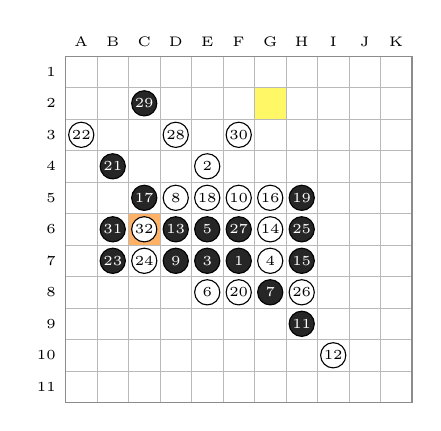
\begin{tikzpicture}[x=0.4cm, y=0.4cm]
\fill[orange!60] (2,-5) rectangle (3,-6);
\fill[yellow!60] (6,-1) rectangle (7,-2);
\draw[gray!55, line width=.3pt, step=1] (0,0) grid (11,-11);
\draw[gray!90] (0,0) rectangle (11,-11);
\node[font=\tiny, anchor=south] at (0.5,0) {A};
\node[font=\tiny, anchor=south] at (1.5,0) {B};
\node[font=\tiny, anchor=south] at (2.5,0) {C};
\node[font=\tiny, anchor=south] at (3.5,0) {D};
\node[font=\tiny, anchor=south] at (4.5,0) {E};
\node[font=\tiny, anchor=south] at (5.5,0) {F};
\node[font=\tiny, anchor=south] at (6.5,0) {G};
\node[font=\tiny, anchor=south] at (7.5,0) {H};
\node[font=\tiny, anchor=south] at (8.5,0) {I};
\node[font=\tiny, anchor=south] at (9.5,0) {J};
\node[font=\tiny, anchor=south] at (10.5,0) {K};
\node[font=\tiny, anchor=east] at (0,-0.5) {1};
\node[font=\tiny, anchor=east] at (0,-1.5) {2};
\node[font=\tiny, anchor=east] at (0,-2.5) {3};
\node[font=\tiny, anchor=east] at (0,-3.5) {4};
\node[font=\tiny, anchor=east] at (0,-4.5) {5};
\node[font=\tiny, anchor=east] at (0,-5.5) {6};
\node[font=\tiny, anchor=east] at (0,-6.5) {7};
\node[font=\tiny, anchor=east] at (0,-7.5) {8};
\node[font=\tiny, anchor=east] at (0,-8.5) {9};
\node[font=\tiny, anchor=east] at (0,-9.5) {10};
\node[font=\tiny, anchor=east] at (0,-10.5) {11};
\draw[fill=black!85, line width=.4pt] (2.5,-1.5) circle (.40);
\node[font=\tiny, text=white, inner sep=0pt] at (2.5,-1.5) {29};
\draw[fill=white, line width=.4pt] (0.5,-2.5) circle (.40);
\node[font=\tiny, text=black, inner sep=0pt] at (0.5,-2.5) {22};
\draw[fill=white, line width=.4pt] (3.5,-2.5) circle (.40);
\node[font=\tiny, text=black, inner sep=0pt] at (3.5,-2.5) {28};
\draw[fill=white, line width=.4pt] (5.5,-2.5) circle (.40);
\node[font=\tiny, text=black, inner sep=0pt] at (5.5,-2.5) {30};
\draw[fill=black!85, line width=.4pt] (1.5,-3.5) circle (.40);
\node[font=\tiny, text=white, inner sep=0pt] at (1.5,-3.5) {21};
\draw[fill=white, line width=.4pt] (4.5,-3.5) circle (.40);
\node[font=\tiny, text=black, inner sep=0pt] at (4.5,-3.5) {2};
\draw[fill=black!85, line width=.4pt] (2.5,-4.5) circle (.40);
\node[font=\tiny, text=white, inner sep=0pt] at (2.5,-4.5) {17};
\draw[fill=white, line width=.4pt] (3.5,-4.5) circle (.40);
\node[font=\tiny, text=black, inner sep=0pt] at (3.5,-4.5) {8};
\draw[fill=white, line width=.4pt] (4.5,-4.5) circle (.40);
\node[font=\tiny, text=black, inner sep=0pt] at (4.5,-4.5) {18};
\draw[fill=white, line width=.4pt] (5.5,-4.5) circle (.40);
\node[font=\tiny, text=black, inner sep=0pt] at (5.5,-4.5) {10};
\draw[fill=white, line width=.4pt] (6.5,-4.5) circle (.40);
\node[font=\tiny, text=black, inner sep=0pt] at (6.5,-4.5) {16};
\draw[fill=black!85, line width=.4pt] (7.5,-4.5) circle (.40);
\node[font=\tiny, text=white, inner sep=0pt] at (7.5,-4.5) {19};
\draw[fill=black!85, line width=.4pt] (1.5,-5.5) circle (.40);
\node[font=\tiny, text=white, inner sep=0pt] at (1.5,-5.5) {31};
\draw[fill=white, line width=.4pt] (2.5,-5.5) circle (.40);
\node[font=\tiny, text=black, inner sep=0pt] at (2.5,-5.5) {32};
\draw[fill=black!85, line width=.4pt] (3.5,-5.5) circle (.40);
\node[font=\tiny, text=white, inner sep=0pt] at (3.5,-5.5) {13};
\draw[fill=black!85, line width=.4pt] (4.5,-5.5) circle (.40);
\node[font=\tiny, text=white, inner sep=0pt] at (4.5,-5.5) {5};
\draw[fill=black!85, line width=.4pt] (5.5,-5.5) circle (.40);
\node[font=\tiny, text=white, inner sep=0pt] at (5.5,-5.5) {27};
\draw[fill=white, line width=.4pt] (6.5,-5.5) circle (.40);
\node[font=\tiny, text=black, inner sep=0pt] at (6.5,-5.5) {14};
\draw[fill=black!85, line width=.4pt] (7.5,-5.5) circle (.40);
\node[font=\tiny, text=white, inner sep=0pt] at (7.5,-5.5) {25};
\draw[fill=black!85, line width=.4pt] (1.5,-6.5) circle (.40);
\node[font=\tiny, text=white, inner sep=0pt] at (1.5,-6.5) {23};
\draw[fill=white, line width=.4pt] (2.5,-6.5) circle (.40);
\node[font=\tiny, text=black, inner sep=0pt] at (2.5,-6.5) {24};
\draw[fill=black!85, line width=.4pt] (3.5,-6.5) circle (.40);
\node[font=\tiny, text=white, inner sep=0pt] at (3.5,-6.5) {9};
\draw[fill=black!85, line width=.4pt] (4.5,-6.5) circle (.40);
\node[font=\tiny, text=white, inner sep=0pt] at (4.5,-6.5) {3};
\draw[fill=black!85, line width=.4pt] (5.5,-6.5) circle (.40);
\node[font=\tiny, text=white, inner sep=0pt] at (5.5,-6.5) {1};
\draw[fill=white, line width=.4pt] (6.5,-6.5) circle (.40);
\node[font=\tiny, text=black, inner sep=0pt] at (6.5,-6.5) {4};
\draw[fill=black!85, line width=.4pt] (7.5,-6.5) circle (.40);
\node[font=\tiny, text=white, inner sep=0pt] at (7.5,-6.5) {15};
\draw[fill=white, line width=.4pt] (4.5,-7.5) circle (.40);
\node[font=\tiny, text=black, inner sep=0pt] at (4.5,-7.5) {6};
\draw[fill=white, line width=.4pt] (5.5,-7.5) circle (.40);
\node[font=\tiny, text=black, inner sep=0pt] at (5.5,-7.5) {20};
\draw[fill=black!85, line width=.4pt] (6.5,-7.5) circle (.40);
\node[font=\tiny, text=white, inner sep=0pt] at (6.5,-7.5) {7};
\draw[fill=white, line width=.4pt] (7.5,-7.5) circle (.40);
\node[font=\tiny, text=black, inner sep=0pt] at (7.5,-7.5) {26};
\draw[fill=black!85, line width=.4pt] (7.5,-8.5) circle (.40);
\node[font=\tiny, text=white, inner sep=0pt] at (7.5,-8.5) {11};
\draw[fill=white, line width=.4pt] (8.5,-9.5) circle (.40);
\node[font=\tiny, text=black, inner sep=0pt] at (8.5,-9.5) {12};
\end{tikzpicture}
    \caption{Sau nước 32 (ô cam); ô vàng là điểm đe doạ nó tạo ra}
  \end{subfigure}
  \par\medskip
  \begin{subfigure}[t]{.48\linewidth}
    \centering
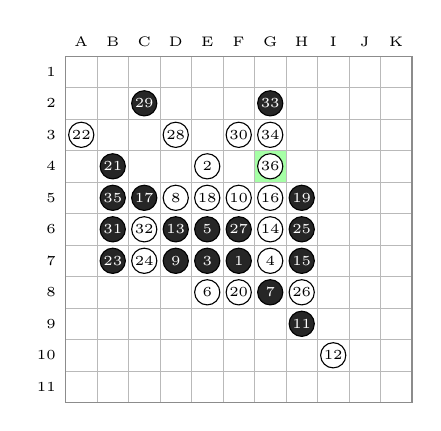
\begin{tikzpicture}[x=0.4cm, y=0.4cm]
\fill[green!35] (6,-3) rectangle (7,-4);
\draw[gray!55, line width=.3pt, step=1] (0,0) grid (11,-11);
\draw[gray!90] (0,0) rectangle (11,-11);
\node[font=\tiny, anchor=south] at (0.5,0) {A};
\node[font=\tiny, anchor=south] at (1.5,0) {B};
\node[font=\tiny, anchor=south] at (2.5,0) {C};
\node[font=\tiny, anchor=south] at (3.5,0) {D};
\node[font=\tiny, anchor=south] at (4.5,0) {E};
\node[font=\tiny, anchor=south] at (5.5,0) {F};
\node[font=\tiny, anchor=south] at (6.5,0) {G};
\node[font=\tiny, anchor=south] at (7.5,0) {H};
\node[font=\tiny, anchor=south] at (8.5,0) {I};
\node[font=\tiny, anchor=south] at (9.5,0) {J};
\node[font=\tiny, anchor=south] at (10.5,0) {K};
\node[font=\tiny, anchor=east] at (0,-0.5) {1};
\node[font=\tiny, anchor=east] at (0,-1.5) {2};
\node[font=\tiny, anchor=east] at (0,-2.5) {3};
\node[font=\tiny, anchor=east] at (0,-3.5) {4};
\node[font=\tiny, anchor=east] at (0,-4.5) {5};
\node[font=\tiny, anchor=east] at (0,-5.5) {6};
\node[font=\tiny, anchor=east] at (0,-6.5) {7};
\node[font=\tiny, anchor=east] at (0,-7.5) {8};
\node[font=\tiny, anchor=east] at (0,-8.5) {9};
\node[font=\tiny, anchor=east] at (0,-9.5) {10};
\node[font=\tiny, anchor=east] at (0,-10.5) {11};
\draw[fill=black!85, line width=.4pt] (2.5,-1.5) circle (.40);
\node[font=\tiny, text=white, inner sep=0pt] at (2.5,-1.5) {29};
\draw[fill=black!85, line width=.4pt] (6.5,-1.5) circle (.40);
\node[font=\tiny, text=white, inner sep=0pt] at (6.5,-1.5) {33};
\draw[fill=white, line width=.4pt] (0.5,-2.5) circle (.40);
\node[font=\tiny, text=black, inner sep=0pt] at (0.5,-2.5) {22};
\draw[fill=white, line width=.4pt] (3.5,-2.5) circle (.40);
\node[font=\tiny, text=black, inner sep=0pt] at (3.5,-2.5) {28};
\draw[fill=white, line width=.4pt] (5.5,-2.5) circle (.40);
\node[font=\tiny, text=black, inner sep=0pt] at (5.5,-2.5) {30};
\draw[fill=white, line width=.4pt] (6.5,-2.5) circle (.40);
\node[font=\tiny, text=black, inner sep=0pt] at (6.5,-2.5) {34};
\draw[fill=black!85, line width=.4pt] (1.5,-3.5) circle (.40);
\node[font=\tiny, text=white, inner sep=0pt] at (1.5,-3.5) {21};
\draw[fill=white, line width=.4pt] (4.5,-3.5) circle (.40);
\node[font=\tiny, text=black, inner sep=0pt] at (4.5,-3.5) {2};
\draw[fill=white, line width=.4pt] (6.5,-3.5) circle (.40);
\node[font=\tiny, text=black, inner sep=0pt] at (6.5,-3.5) {36};
\draw[fill=black!85, line width=.4pt] (1.5,-4.5) circle (.40);
\node[font=\tiny, text=white, inner sep=0pt] at (1.5,-4.5) {35};
\draw[fill=black!85, line width=.4pt] (2.5,-4.5) circle (.40);
\node[font=\tiny, text=white, inner sep=0pt] at (2.5,-4.5) {17};
\draw[fill=white, line width=.4pt] (3.5,-4.5) circle (.40);
\node[font=\tiny, text=black, inner sep=0pt] at (3.5,-4.5) {8};
\draw[fill=white, line width=.4pt] (4.5,-4.5) circle (.40);
\node[font=\tiny, text=black, inner sep=0pt] at (4.5,-4.5) {18};
\draw[fill=white, line width=.4pt] (5.5,-4.5) circle (.40);
\node[font=\tiny, text=black, inner sep=0pt] at (5.5,-4.5) {10};
\draw[fill=white, line width=.4pt] (6.5,-4.5) circle (.40);
\node[font=\tiny, text=black, inner sep=0pt] at (6.5,-4.5) {16};
\draw[fill=black!85, line width=.4pt] (7.5,-4.5) circle (.40);
\node[font=\tiny, text=white, inner sep=0pt] at (7.5,-4.5) {19};
\draw[fill=black!85, line width=.4pt] (1.5,-5.5) circle (.40);
\node[font=\tiny, text=white, inner sep=0pt] at (1.5,-5.5) {31};
\draw[fill=white, line width=.4pt] (2.5,-5.5) circle (.40);
\node[font=\tiny, text=black, inner sep=0pt] at (2.5,-5.5) {32};
\draw[fill=black!85, line width=.4pt] (3.5,-5.5) circle (.40);
\node[font=\tiny, text=white, inner sep=0pt] at (3.5,-5.5) {13};
\draw[fill=black!85, line width=.4pt] (4.5,-5.5) circle (.40);
\node[font=\tiny, text=white, inner sep=0pt] at (4.5,-5.5) {5};
\draw[fill=black!85, line width=.4pt] (5.5,-5.5) circle (.40);
\node[font=\tiny, text=white, inner sep=0pt] at (5.5,-5.5) {27};
\draw[fill=white, line width=.4pt] (6.5,-5.5) circle (.40);
\node[font=\tiny, text=black, inner sep=0pt] at (6.5,-5.5) {14};
\draw[fill=black!85, line width=.4pt] (7.5,-5.5) circle (.40);
\node[font=\tiny, text=white, inner sep=0pt] at (7.5,-5.5) {25};
\draw[fill=black!85, line width=.4pt] (1.5,-6.5) circle (.40);
\node[font=\tiny, text=white, inner sep=0pt] at (1.5,-6.5) {23};
\draw[fill=white, line width=.4pt] (2.5,-6.5) circle (.40);
\node[font=\tiny, text=black, inner sep=0pt] at (2.5,-6.5) {24};
\draw[fill=black!85, line width=.4pt] (3.5,-6.5) circle (.40);
\node[font=\tiny, text=white, inner sep=0pt] at (3.5,-6.5) {9};
\draw[fill=black!85, line width=.4pt] (4.5,-6.5) circle (.40);
\node[font=\tiny, text=white, inner sep=0pt] at (4.5,-6.5) {3};
\draw[fill=black!85, line width=.4pt] (5.5,-6.5) circle (.40);
\node[font=\tiny, text=white, inner sep=0pt] at (5.5,-6.5) {1};
\draw[fill=white, line width=.4pt] (6.5,-6.5) circle (.40);
\node[font=\tiny, text=black, inner sep=0pt] at (6.5,-6.5) {4};
\draw[fill=black!85, line width=.4pt] (7.5,-6.5) circle (.40);
\node[font=\tiny, text=white, inner sep=0pt] at (7.5,-6.5) {15};
\draw[fill=white, line width=.4pt] (4.5,-7.5) circle (.40);
\node[font=\tiny, text=black, inner sep=0pt] at (4.5,-7.5) {6};
\draw[fill=white, line width=.4pt] (5.5,-7.5) circle (.40);
\node[font=\tiny, text=black, inner sep=0pt] at (5.5,-7.5) {20};
\draw[fill=black!85, line width=.4pt] (6.5,-7.5) circle (.40);
\node[font=\tiny, text=white, inner sep=0pt] at (6.5,-7.5) {7};
\draw[fill=white, line width=.4pt] (7.5,-7.5) circle (.40);
\node[font=\tiny, text=black, inner sep=0pt] at (7.5,-7.5) {26};
\draw[fill=black!85, line width=.4pt] (7.5,-8.5) circle (.40);
\node[font=\tiny, text=white, inner sep=0pt] at (7.5,-8.5) {11};
\draw[fill=white, line width=.4pt] (8.5,-9.5) circle (.40);
\node[font=\tiny, text=black, inner sep=0pt] at (8.5,-9.5) {12};
\end{tikzpicture}
    \caption{Thế cuối (ô xanh: nước kết thúc)}
  \end{subfigure}
  \par\medskip
  \caption{Ván 13: X là L7, O là L8, L8 thắng. Số trên quân là thứ tự nước.}
  \label{fig:cs-vs-13}
\end{figure}

\paragraph{Diễn biến.} Đây là ván đổi chiều nhiều lần.
\begin{itemize}
  \item \textbf{Nước 9 (X, D7):} điểm của X rơi từ $95\%$ xuống $36\%$. KataGomo đề nghị F9. L7 đánh mất phần lớn lợi thế
  khai cuộc.
  \item \textbf{Nước 13 và 15 (X):} D6 rồi H7 đưa điểm của X xuống còn $1\%$. Lúc này L8 đang thắng theo engine.
  \item \textbf{Nước 16 (O, G5):} sai lầm lớn nhất của L8 theo engine, điểm của X bật từ $1\%$ lên $96\%$. G5 tạo ba hở
  ngang nhưng bỏ ô C5; ngay nước 17 L7 chiếm đúng C5 và dựng ba hở chéo xuôi của mình.
  \item \textbf{Nước 17--24:} L7 giữ thế chủ động; L8 chủ yếu phải đỡ, chỉ xen được một phản tứ ở nước 18.
  \item \textbf{Nước 25 (X, H6):} L7 đi một nước tứ mà engine đánh giá là sai. Ô chặn H8 mà O buộc phải đi lại cho O một ba hở
  chéo xuôi, trả quyền chủ động; điểm của X từ $100\%$ xuống $48\%$. KataGomo đề nghị B6.
  \item \textbf{Nước 26--30:} thế cân bằng, engine báo tỷ lệ hoà cao.
\end{itemize}
Các nhận định trên dựa vào KataGomo; trong đoạn này bộ giải (độ sâu 2) không chứng minh được đường thắng ép nào.

\paragraph{Sai lầm quyết định: nước 31 (X, B6).} B6 là một nước tứ, buộc O phải chặn tại C6. Nhưng C6 đồng thời tạo cho
O \emph{một tứ chéo ngược} (đe doạ G2). Quyền chủ động đổi sang O đúng ở lượt O buộc phải đỡ. Từ nước 32, bộ giải chứng
minh O thắng bằng chuỗi tứ C6--G2--G3--G4--E3--C3--H3. Ba ô tránh được trong độ sâu của bộ giải là H3, H4 và C6 (chiếm
luôn ô mà nước tứ sẽ biếu cho đối thủ). KataGomo cũng đề nghị C6; điểm của X trước nước 31 là $44\%$, sau B6 là $0\%$.

\paragraph{Vì sao L8 thắng.} Nước 32 vừa đỡ vừa công. L7 buộc đỡ G2 (nước 33); nước 34 (G3) tạo cùng lúc một ba hở
ngang và một tứ dọc. L7 đi B5 để dựng tứ của mình ở nước 35, nhưng O đến lượt trước và hoàn thành năm quân tại G4.
Nước 35 (không chặn G4) trông như lỗi thua ván, nhưng ván đã thua từ nước 31: ngay cả khi
chặn G4, chuỗi tứ đã chứng minh vẫn tiếp tục qua E3, C3 và H3.
\par{\scriptsize
\renewcommand{\arraystretch}{0.95}
\begin{longtable}{rlp{4.4cm}lrll}
  \caption{Diễn biến ván 13 sau khai cuộc}\label{tab:cs-vs-13}\\
    \toprule
    Nước & Đi & Hình tạo / đỡ & Thắng ép & X \% & KG &  \\
    \midrule
  \endfirsthead
    \toprule
    Nước & Đi & Hình tạo / đỡ & Thắng ép & X \% & KG &  \\
    \midrule
  \endhead
    \bottomrule
  \endfoot
    3 & X E7 & --- & --- & 94 & E6 &  \\
    4 & O G7 & --- & --- & 91 & H7 &  \\
    5 & X E6 & --- & --- & 96 & E8 &  \\
    6 & O E8 & --- & --- & 95 & B7 &  \\
    7 & X G8 & ba hở chéo xuôi & --- & 96 & D7 &  \\
    8 & O D5 & chặn đòn kép & --- & 95 & D5 &  \\
    9 & X D7 & --- & --- & 95 & F9 &  \\
    10 & O F5 & --- & --- & 36 & F5 &  \\
    11 & X H9 & tứ chéo xuôi & --- & 20 & H9 &  \\
    12 & O I10 & chặn năm & --- & 23 & I10 &  \\
    13 & X D6 & --- & --- & 25 & C5 &  \\
    14 & O G6 & ba hở chéo xuôi & --- & 4 & C5 &  \\
    15 & X H7 & chặn đòn kép & --- & 19 & D3 &  \\
    16 & O G5 & ba hở ngang & --- & 1 & C5 &  \\
    17 & X C5 & ba hở chéo xuôi & --- & 96 & C5 &  \\
    18 & O E5 & tứ ngang & --- & 97 & F8 &  \\
    19 & X H5 & chặn năm & --- & 99 & H5 &  \\
    20 & O F8 & chặn đòn kép & --- & 100 & B4 &  \\
    21 & X B4 & tứ chéo xuôi & --- & 100 & B6 &  \\
    22 & O A3 & chặn năm & --- & 100 & A3 &  \\
    23 & X B7 & tứ ngang & --- & 100 & B6 &  \\
    24 & O C7 & chặn năm & --- & 100 & C7 &  \\
    25 & X H6 & tứ dọc & --- & 100 & B6 &  \\
    26 & O H8 & chặn năm, ba hở chéo xuôi & --- & 48 & H8 &  \\
    27 & X F6 & chặn đòn kép & --- & 47 & F6 &  \\
    28 & O D3 & tứ chéo xuôi & --- & 49 & F3 &  \\
    29 & X C2 & chặn năm & --- & 47 & C2 &  \\
    30 & O F3 & ba hở chéo ngược & --- & 47 & F3 &  \\
    31 & X B6 & tứ ngang, ba hở dọc & --- & 44 & C6 & \textbf{sai lầm} \\
    32 & O C6 & chặn năm, tứ chéo ngược & VCF (C6) & 0 & C6 & \textbf{khoá ván} \\
    33 & X G2 & chặn năm & --- & 0 & G2 &  \\
    34 & O G3 & ba hở ngang, tứ dọc & VCF (G3) & 0 & G3 &  \\
    35 & X B5 & tứ hở dọc & --- & 0 & G4 &  \\
    36 & O G4 & chặn đòn kép, năm dọc & VCF (G4) & 0 & G4 &  \\
\end{longtable}
}


\subsection{Ván 26: L3 thắng L8 bằng năm ba hở liên tiếp}
\label{sec:cs-vs-26}
L3 (Alpha-Beta) cầm X, L8 cầm O, khai cuộc H5--F8--G7. Trước nước 4, KataGomo chấm X $82\%$.
\begin{figure}[!htbp]
  \centering
  \begin{subfigure}[t]{.48\linewidth}
    \centering
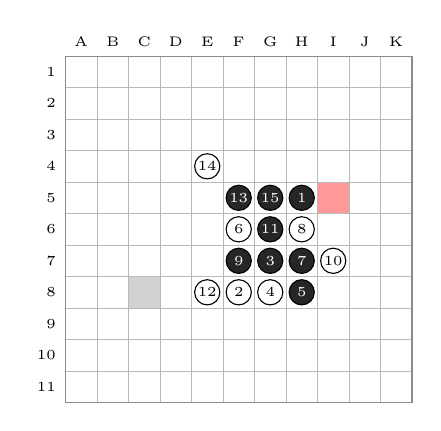
\begin{tikzpicture}[x=0.4cm, y=0.4cm]
\fill[gray!35] (2,-7) rectangle (3,-8);
\fill[red!40] (8,-4) rectangle (9,-5);
\draw[gray!55, line width=.3pt, step=1] (0,0) grid (11,-11);
\draw[gray!90] (0,0) rectangle (11,-11);
\node[font=\tiny, anchor=south] at (0.5,0) {A};
\node[font=\tiny, anchor=south] at (1.5,0) {B};
\node[font=\tiny, anchor=south] at (2.5,0) {C};
\node[font=\tiny, anchor=south] at (3.5,0) {D};
\node[font=\tiny, anchor=south] at (4.5,0) {E};
\node[font=\tiny, anchor=south] at (5.5,0) {F};
\node[font=\tiny, anchor=south] at (6.5,0) {G};
\node[font=\tiny, anchor=south] at (7.5,0) {H};
\node[font=\tiny, anchor=south] at (8.5,0) {I};
\node[font=\tiny, anchor=south] at (9.5,0) {J};
\node[font=\tiny, anchor=south] at (10.5,0) {K};
\node[font=\tiny, anchor=east] at (0,-0.5) {1};
\node[font=\tiny, anchor=east] at (0,-1.5) {2};
\node[font=\tiny, anchor=east] at (0,-2.5) {3};
\node[font=\tiny, anchor=east] at (0,-3.5) {4};
\node[font=\tiny, anchor=east] at (0,-4.5) {5};
\node[font=\tiny, anchor=east] at (0,-5.5) {6};
\node[font=\tiny, anchor=east] at (0,-6.5) {7};
\node[font=\tiny, anchor=east] at (0,-7.5) {8};
\node[font=\tiny, anchor=east] at (0,-8.5) {9};
\node[font=\tiny, anchor=east] at (0,-9.5) {10};
\node[font=\tiny, anchor=east] at (0,-10.5) {11};
\draw[fill=white, line width=.4pt] (4.5,-3.5) circle (.40);
\node[font=\tiny, text=black, inner sep=0pt] at (4.5,-3.5) {14};
\draw[fill=black!85, line width=.4pt] (5.5,-4.5) circle (.40);
\node[font=\tiny, text=white, inner sep=0pt] at (5.5,-4.5) {13};
\draw[fill=black!85, line width=.4pt] (6.5,-4.5) circle (.40);
\node[font=\tiny, text=white, inner sep=0pt] at (6.5,-4.5) {15};
\draw[fill=black!85, line width=.4pt] (7.5,-4.5) circle (.40);
\node[font=\tiny, text=white, inner sep=0pt] at (7.5,-4.5) {1};
\draw[fill=white, line width=.4pt] (5.5,-5.5) circle (.40);
\node[font=\tiny, text=black, inner sep=0pt] at (5.5,-5.5) {6};
\draw[fill=black!85, line width=.4pt] (6.5,-5.5) circle (.40);
\node[font=\tiny, text=white, inner sep=0pt] at (6.5,-5.5) {11};
\draw[fill=white, line width=.4pt] (7.5,-5.5) circle (.40);
\node[font=\tiny, text=black, inner sep=0pt] at (7.5,-5.5) {8};
\draw[fill=black!85, line width=.4pt] (5.5,-6.5) circle (.40);
\node[font=\tiny, text=white, inner sep=0pt] at (5.5,-6.5) {9};
\draw[fill=black!85, line width=.4pt] (6.5,-6.5) circle (.40);
\node[font=\tiny, text=white, inner sep=0pt] at (6.5,-6.5) {3};
\draw[fill=black!85, line width=.4pt] (7.5,-6.5) circle (.40);
\node[font=\tiny, text=white, inner sep=0pt] at (7.5,-6.5) {7};
\draw[fill=white, line width=.4pt] (8.5,-6.5) circle (.40);
\node[font=\tiny, text=black, inner sep=0pt] at (8.5,-6.5) {10};
\draw[fill=white, line width=.4pt] (4.5,-7.5) circle (.40);
\node[font=\tiny, text=black, inner sep=0pt] at (4.5,-7.5) {12};
\draw[fill=white, line width=.4pt] (5.5,-7.5) circle (.40);
\node[font=\tiny, text=black, inner sep=0pt] at (5.5,-7.5) {2};
\draw[fill=white, line width=.4pt] (6.5,-7.5) circle (.40);
\node[font=\tiny, text=black, inner sep=0pt] at (6.5,-7.5) {4};
\draw[fill=black!85, line width=.4pt] (7.5,-7.5) circle (.40);
\node[font=\tiny, text=white, inner sep=0pt] at (7.5,-7.5) {5};
\end{tikzpicture}
    \caption{Trước nước 16: ô đỏ là nước đã đi; 1 ô xám chỉ hoãn thua, không cứu được}
  \end{subfigure}
  \hfill
  \begin{subfigure}[t]{.48\linewidth}
    \centering
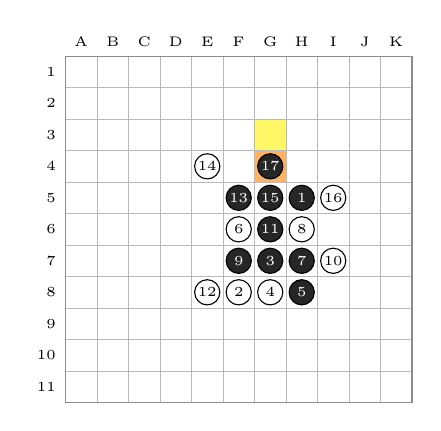
\begin{tikzpicture}[x=0.4cm, y=0.4cm]
\fill[orange!60] (6,-3) rectangle (7,-4);
\fill[yellow!60] (6,-2) rectangle (7,-3);
\draw[gray!55, line width=.3pt, step=1] (0,0) grid (11,-11);
\draw[gray!90] (0,0) rectangle (11,-11);
\node[font=\tiny, anchor=south] at (0.5,0) {A};
\node[font=\tiny, anchor=south] at (1.5,0) {B};
\node[font=\tiny, anchor=south] at (2.5,0) {C};
\node[font=\tiny, anchor=south] at (3.5,0) {D};
\node[font=\tiny, anchor=south] at (4.5,0) {E};
\node[font=\tiny, anchor=south] at (5.5,0) {F};
\node[font=\tiny, anchor=south] at (6.5,0) {G};
\node[font=\tiny, anchor=south] at (7.5,0) {H};
\node[font=\tiny, anchor=south] at (8.5,0) {I};
\node[font=\tiny, anchor=south] at (9.5,0) {J};
\node[font=\tiny, anchor=south] at (10.5,0) {K};
\node[font=\tiny, anchor=east] at (0,-0.5) {1};
\node[font=\tiny, anchor=east] at (0,-1.5) {2};
\node[font=\tiny, anchor=east] at (0,-2.5) {3};
\node[font=\tiny, anchor=east] at (0,-3.5) {4};
\node[font=\tiny, anchor=east] at (0,-4.5) {5};
\node[font=\tiny, anchor=east] at (0,-5.5) {6};
\node[font=\tiny, anchor=east] at (0,-6.5) {7};
\node[font=\tiny, anchor=east] at (0,-7.5) {8};
\node[font=\tiny, anchor=east] at (0,-8.5) {9};
\node[font=\tiny, anchor=east] at (0,-9.5) {10};
\node[font=\tiny, anchor=east] at (0,-10.5) {11};
\draw[fill=white, line width=.4pt] (4.5,-3.5) circle (.40);
\node[font=\tiny, text=black, inner sep=0pt] at (4.5,-3.5) {14};
\draw[fill=black!85, line width=.4pt] (6.5,-3.5) circle (.40);
\node[font=\tiny, text=white, inner sep=0pt] at (6.5,-3.5) {17};
\draw[fill=black!85, line width=.4pt] (5.5,-4.5) circle (.40);
\node[font=\tiny, text=white, inner sep=0pt] at (5.5,-4.5) {13};
\draw[fill=black!85, line width=.4pt] (6.5,-4.5) circle (.40);
\node[font=\tiny, text=white, inner sep=0pt] at (6.5,-4.5) {15};
\draw[fill=black!85, line width=.4pt] (7.5,-4.5) circle (.40);
\node[font=\tiny, text=white, inner sep=0pt] at (7.5,-4.5) {1};
\draw[fill=white, line width=.4pt] (8.5,-4.5) circle (.40);
\node[font=\tiny, text=black, inner sep=0pt] at (8.5,-4.5) {16};
\draw[fill=white, line width=.4pt] (5.5,-5.5) circle (.40);
\node[font=\tiny, text=black, inner sep=0pt] at (5.5,-5.5) {6};
\draw[fill=black!85, line width=.4pt] (6.5,-5.5) circle (.40);
\node[font=\tiny, text=white, inner sep=0pt] at (6.5,-5.5) {11};
\draw[fill=white, line width=.4pt] (7.5,-5.5) circle (.40);
\node[font=\tiny, text=black, inner sep=0pt] at (7.5,-5.5) {8};
\draw[fill=black!85, line width=.4pt] (5.5,-6.5) circle (.40);
\node[font=\tiny, text=white, inner sep=0pt] at (5.5,-6.5) {9};
\draw[fill=black!85, line width=.4pt] (6.5,-6.5) circle (.40);
\node[font=\tiny, text=white, inner sep=0pt] at (6.5,-6.5) {3};
\draw[fill=black!85, line width=.4pt] (7.5,-6.5) circle (.40);
\node[font=\tiny, text=white, inner sep=0pt] at (7.5,-6.5) {7};
\draw[fill=white, line width=.4pt] (8.5,-6.5) circle (.40);
\node[font=\tiny, text=black, inner sep=0pt] at (8.5,-6.5) {10};
\draw[fill=white, line width=.4pt] (4.5,-7.5) circle (.40);
\node[font=\tiny, text=black, inner sep=0pt] at (4.5,-7.5) {12};
\draw[fill=white, line width=.4pt] (5.5,-7.5) circle (.40);
\node[font=\tiny, text=black, inner sep=0pt] at (5.5,-7.5) {2};
\draw[fill=white, line width=.4pt] (6.5,-7.5) circle (.40);
\node[font=\tiny, text=black, inner sep=0pt] at (6.5,-7.5) {4};
\draw[fill=black!85, line width=.4pt] (7.5,-7.5) circle (.40);
\node[font=\tiny, text=white, inner sep=0pt] at (7.5,-7.5) {5};
\end{tikzpicture}
    \caption{Sau nước 17 (ô cam); ô vàng là điểm đe doạ nó tạo ra}
  \end{subfigure}
  \par\medskip
  \begin{subfigure}[t]{.48\linewidth}
    \centering
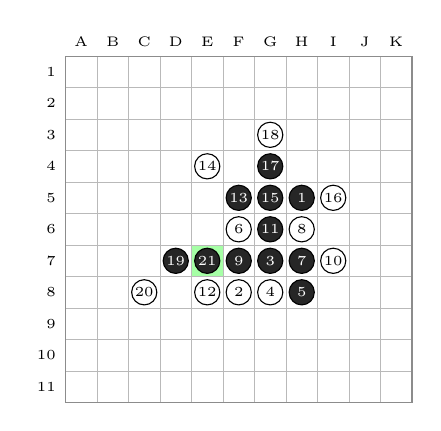
\begin{tikzpicture}[x=0.4cm, y=0.4cm]
\fill[green!35] (4,-6) rectangle (5,-7);
\draw[gray!55, line width=.3pt, step=1] (0,0) grid (11,-11);
\draw[gray!90] (0,0) rectangle (11,-11);
\node[font=\tiny, anchor=south] at (0.5,0) {A};
\node[font=\tiny, anchor=south] at (1.5,0) {B};
\node[font=\tiny, anchor=south] at (2.5,0) {C};
\node[font=\tiny, anchor=south] at (3.5,0) {D};
\node[font=\tiny, anchor=south] at (4.5,0) {E};
\node[font=\tiny, anchor=south] at (5.5,0) {F};
\node[font=\tiny, anchor=south] at (6.5,0) {G};
\node[font=\tiny, anchor=south] at (7.5,0) {H};
\node[font=\tiny, anchor=south] at (8.5,0) {I};
\node[font=\tiny, anchor=south] at (9.5,0) {J};
\node[font=\tiny, anchor=south] at (10.5,0) {K};
\node[font=\tiny, anchor=east] at (0,-0.5) {1};
\node[font=\tiny, anchor=east] at (0,-1.5) {2};
\node[font=\tiny, anchor=east] at (0,-2.5) {3};
\node[font=\tiny, anchor=east] at (0,-3.5) {4};
\node[font=\tiny, anchor=east] at (0,-4.5) {5};
\node[font=\tiny, anchor=east] at (0,-5.5) {6};
\node[font=\tiny, anchor=east] at (0,-6.5) {7};
\node[font=\tiny, anchor=east] at (0,-7.5) {8};
\node[font=\tiny, anchor=east] at (0,-8.5) {9};
\node[font=\tiny, anchor=east] at (0,-9.5) {10};
\node[font=\tiny, anchor=east] at (0,-10.5) {11};
\draw[fill=white, line width=.4pt] (6.5,-2.5) circle (.40);
\node[font=\tiny, text=black, inner sep=0pt] at (6.5,-2.5) {18};
\draw[fill=white, line width=.4pt] (4.5,-3.5) circle (.40);
\node[font=\tiny, text=black, inner sep=0pt] at (4.5,-3.5) {14};
\draw[fill=black!85, line width=.4pt] (6.5,-3.5) circle (.40);
\node[font=\tiny, text=white, inner sep=0pt] at (6.5,-3.5) {17};
\draw[fill=black!85, line width=.4pt] (5.5,-4.5) circle (.40);
\node[font=\tiny, text=white, inner sep=0pt] at (5.5,-4.5) {13};
\draw[fill=black!85, line width=.4pt] (6.5,-4.5) circle (.40);
\node[font=\tiny, text=white, inner sep=0pt] at (6.5,-4.5) {15};
\draw[fill=black!85, line width=.4pt] (7.5,-4.5) circle (.40);
\node[font=\tiny, text=white, inner sep=0pt] at (7.5,-4.5) {1};
\draw[fill=white, line width=.4pt] (8.5,-4.5) circle (.40);
\node[font=\tiny, text=black, inner sep=0pt] at (8.5,-4.5) {16};
\draw[fill=white, line width=.4pt] (5.5,-5.5) circle (.40);
\node[font=\tiny, text=black, inner sep=0pt] at (5.5,-5.5) {6};
\draw[fill=black!85, line width=.4pt] (6.5,-5.5) circle (.40);
\node[font=\tiny, text=white, inner sep=0pt] at (6.5,-5.5) {11};
\draw[fill=white, line width=.4pt] (7.5,-5.5) circle (.40);
\node[font=\tiny, text=black, inner sep=0pt] at (7.5,-5.5) {8};
\draw[fill=black!85, line width=.4pt] (3.5,-6.5) circle (.40);
\node[font=\tiny, text=white, inner sep=0pt] at (3.5,-6.5) {19};
\draw[fill=black!85, line width=.4pt] (4.5,-6.5) circle (.40);
\node[font=\tiny, text=white, inner sep=0pt] at (4.5,-6.5) {21};
\draw[fill=black!85, line width=.4pt] (5.5,-6.5) circle (.40);
\node[font=\tiny, text=white, inner sep=0pt] at (5.5,-6.5) {9};
\draw[fill=black!85, line width=.4pt] (6.5,-6.5) circle (.40);
\node[font=\tiny, text=white, inner sep=0pt] at (6.5,-6.5) {3};
\draw[fill=black!85, line width=.4pt] (7.5,-6.5) circle (.40);
\node[font=\tiny, text=white, inner sep=0pt] at (7.5,-6.5) {7};
\draw[fill=white, line width=.4pt] (8.5,-6.5) circle (.40);
\node[font=\tiny, text=black, inner sep=0pt] at (8.5,-6.5) {10};
\draw[fill=white, line width=.4pt] (2.5,-7.5) circle (.40);
\node[font=\tiny, text=black, inner sep=0pt] at (2.5,-7.5) {20};
\draw[fill=white, line width=.4pt] (4.5,-7.5) circle (.40);
\node[font=\tiny, text=black, inner sep=0pt] at (4.5,-7.5) {12};
\draw[fill=white, line width=.4pt] (5.5,-7.5) circle (.40);
\node[font=\tiny, text=black, inner sep=0pt] at (5.5,-7.5) {2};
\draw[fill=white, line width=.4pt] (6.5,-7.5) circle (.40);
\node[font=\tiny, text=black, inner sep=0pt] at (6.5,-7.5) {4};
\draw[fill=black!85, line width=.4pt] (7.5,-7.5) circle (.40);
\node[font=\tiny, text=white, inner sep=0pt] at (7.5,-7.5) {5};
\end{tikzpicture}
    \caption{Thế cuối (ô xanh: nước kết thúc)}
  \end{subfigure}
  \par\medskip
  \caption{Ván 26: X là L3, O là L8, L3 thắng. Số trên quân là thứ tự nước.}
  \label{fig:cs-vs-26}
\end{figure}

\paragraph{Diễn biến.}
\begin{itemize}
  \item \textbf{Nước 4 (O, G8) và 6 (O, F6):} hai nước của L8 đưa điểm của X từ $82\%$ lên $98\%$; engine đề nghị F7 cả hai
  lần. Đây là chỗ L8 mất điểm; sau đó engine coi ván gần như đã định.
  \item \textbf{Nước 7, 9, 11, 13, 15 (X):} L3 tạo năm ba hở liên tiếp theo cả bốn hướng (H7 dọc, F7 ngang, G6 chéo ngược,
  F5 chéo xuôi, G5 ngang). Mỗi nước buộc L8 đỡ ngay (nước 8, 10, 12, 14, 16 đều là nước chặn đòn kép).
\end{itemize}
\paragraph{Nước 16 và nước khoá ván 17.} L8 chặn một đầu của ba hở ngang tại I5, và từ nước 17 bộ giải chứng minh X thắng
bằng chuỗi tứ G4--G3--D7--E7--E6--H3--C8. Ở độ sâu của bộ giải, chỉ C8 (ô cuối của chuỗi) tránh được chuỗi đó; nhưng khi
tìm sâu hơn một bậc, C8 cũng bị bác bỏ bằng một chuỗi đe doạ mở đầu D8, và engine chấm O $0\%$. Vậy I5 làm ván kết thúc
nhanh hơn, \emph{không phải} nguyên nhân thua.

\paragraph{Vì sao L3 thắng.} L3 không để mất quyền chủ động: từ nước 7, mọi nước của X đều là đe doạ. Nước 17 (G4) tạo tứ
dọc; nước 19 (D7) tạo cùng lúc tứ ngang và ba hở chéo ngược; L8 chặn kèm phản tứ ở nước 20 (C8) nhưng X đến lượt trước
và hoàn thành năm quân tại E7. Việc O đi C8 thay vì chặn E7 ở nước 20 không phải nguyên nhân thua: bộ giải cho thấy
X đã thắng ép từ trước đó, kể cả khi O chặn E7.
\par{\scriptsize
\renewcommand{\arraystretch}{0.95}
\begin{longtable}{rlp{4.4cm}lrll}
  \caption{Diễn biến ván 26 sau khai cuộc}\label{tab:cs-vs-26}\\
    \toprule
    Nước & Đi & Hình tạo / đỡ & Thắng ép & X \% & KG &  \\
    \midrule
  \endfirsthead
    \toprule
    Nước & Đi & Hình tạo / đỡ & Thắng ép & X \% & KG &  \\
    \midrule
  \endhead
    \bottomrule
  \endfoot
    4 & O G8 & --- & --- & 82 & F7 & mất điểm \\
    5 & X H8 & --- & --- & 93 & H8 &  \\
    6 & O F6 & --- & --- & 92 & F7 &  \\
    7 & X H7 & ba hở dọc & --- & 98 & H7 &  \\
    8 & O H6 & chặn đòn kép & --- & 99 & H4 &  \\
    9 & X F7 & ba hở ngang & --- & 99 & F7 &  \\
    10 & O I7 & chặn đòn kép & --- & 100 & I7 &  \\
    11 & X G6 & ba hở chéo ngược & --- & 99 & G6 &  \\
    12 & O E8 & chặn đòn kép & --- & 99 & E8 &  \\
    13 & X F5 & ba hở chéo xuôi & --- & 99 & F5 &  \\
    14 & O E4 & chặn đòn kép & --- & 99 & I8 &  \\
    15 & X G5 & ba hở ngang & --- & 100 & G5 &  \\
    16 & O I5 & chặn đòn kép & --- & 100 & I5 &  \\
    17 & X G4 & tứ dọc & VCF (G4) & 100 & D7 & \textbf{khoá ván} \\
    18 & O G3 & chặn năm & --- & 100 & G3 &  \\
    19 & X D7 & tứ ngang, ba hở chéo ngược & VCF (D7) & 100 & D7 &  \\
    20 & O C8 & chặn đòn kép, tứ ngang & --- & 100 & E7 &  \\
    21 & X E7 & năm ngang & VCF (E7) & 100 & E7 &  \\
\end{longtable}
}


\subsection{Ván 1202: tác tử luật L2 thắng L8}
\label{sec:cs-vs-1202}
L2 cầm X, L8 cầm O, khai cuộc F4--H5--D6--D8. Đây là một trong 7 ván L2 thắng trên 100 ván của cặp. Ngay sau khai cuộc,
KataGomo chấm X $95\%$ và điểm của O không vượt quá vài phần trăm trong cả ván: theo engine, ván đã nghiêng từ thế mở đầu,
trước khi L2 đi nước nào.
\begin{figure}[!htbp]
  \centering
  \begin{subfigure}[t]{.48\linewidth}
    \centering
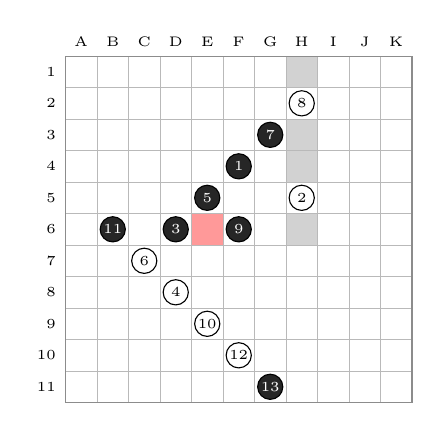
\begin{tikzpicture}[x=0.4cm, y=0.4cm]
\fill[gray!35] (7,0) rectangle (8,-1);
\fill[gray!35] (7,-2) rectangle (8,-3);
\fill[gray!35] (7,-3) rectangle (8,-4);
\fill[gray!35] (7,-5) rectangle (8,-6);
\fill[red!40] (4,-5) rectangle (5,-6);
\draw[gray!55, line width=.3pt, step=1] (0,0) grid (11,-11);
\draw[gray!90] (0,0) rectangle (11,-11);
\node[font=\tiny, anchor=south] at (0.5,0) {A};
\node[font=\tiny, anchor=south] at (1.5,0) {B};
\node[font=\tiny, anchor=south] at (2.5,0) {C};
\node[font=\tiny, anchor=south] at (3.5,0) {D};
\node[font=\tiny, anchor=south] at (4.5,0) {E};
\node[font=\tiny, anchor=south] at (5.5,0) {F};
\node[font=\tiny, anchor=south] at (6.5,0) {G};
\node[font=\tiny, anchor=south] at (7.5,0) {H};
\node[font=\tiny, anchor=south] at (8.5,0) {I};
\node[font=\tiny, anchor=south] at (9.5,0) {J};
\node[font=\tiny, anchor=south] at (10.5,0) {K};
\node[font=\tiny, anchor=east] at (0,-0.5) {1};
\node[font=\tiny, anchor=east] at (0,-1.5) {2};
\node[font=\tiny, anchor=east] at (0,-2.5) {3};
\node[font=\tiny, anchor=east] at (0,-3.5) {4};
\node[font=\tiny, anchor=east] at (0,-4.5) {5};
\node[font=\tiny, anchor=east] at (0,-5.5) {6};
\node[font=\tiny, anchor=east] at (0,-6.5) {7};
\node[font=\tiny, anchor=east] at (0,-7.5) {8};
\node[font=\tiny, anchor=east] at (0,-8.5) {9};
\node[font=\tiny, anchor=east] at (0,-9.5) {10};
\node[font=\tiny, anchor=east] at (0,-10.5) {11};
\draw[fill=white, line width=.4pt] (7.5,-1.5) circle (.40);
\node[font=\tiny, text=black, inner sep=0pt] at (7.5,-1.5) {8};
\draw[fill=black!85, line width=.4pt] (6.5,-2.5) circle (.40);
\node[font=\tiny, text=white, inner sep=0pt] at (6.5,-2.5) {7};
\draw[fill=black!85, line width=.4pt] (5.5,-3.5) circle (.40);
\node[font=\tiny, text=white, inner sep=0pt] at (5.5,-3.5) {1};
\draw[fill=black!85, line width=.4pt] (4.5,-4.5) circle (.40);
\node[font=\tiny, text=white, inner sep=0pt] at (4.5,-4.5) {5};
\draw[fill=white, line width=.4pt] (7.5,-4.5) circle (.40);
\node[font=\tiny, text=black, inner sep=0pt] at (7.5,-4.5) {2};
\draw[fill=black!85, line width=.4pt] (1.5,-5.5) circle (.40);
\node[font=\tiny, text=white, inner sep=0pt] at (1.5,-5.5) {11};
\draw[fill=black!85, line width=.4pt] (3.5,-5.5) circle (.40);
\node[font=\tiny, text=white, inner sep=0pt] at (3.5,-5.5) {3};
\draw[fill=black!85, line width=.4pt] (5.5,-5.5) circle (.40);
\node[font=\tiny, text=white, inner sep=0pt] at (5.5,-5.5) {9};
\draw[fill=white, line width=.4pt] (2.5,-6.5) circle (.40);
\node[font=\tiny, text=black, inner sep=0pt] at (2.5,-6.5) {6};
\draw[fill=white, line width=.4pt] (3.5,-7.5) circle (.40);
\node[font=\tiny, text=black, inner sep=0pt] at (3.5,-7.5) {4};
\draw[fill=white, line width=.4pt] (4.5,-8.5) circle (.40);
\node[font=\tiny, text=black, inner sep=0pt] at (4.5,-8.5) {10};
\draw[fill=white, line width=.4pt] (5.5,-9.5) circle (.40);
\node[font=\tiny, text=black, inner sep=0pt] at (5.5,-9.5) {12};
\draw[fill=black!85, line width=.4pt] (6.5,-10.5) circle (.40);
\node[font=\tiny, text=white, inner sep=0pt] at (6.5,-10.5) {13};
\end{tikzpicture}
    \caption{Trước nước 14: ô đỏ là nước đã đi; 4 ô xám chỉ hoãn thua, không cứu được}
  \end{subfigure}
  \hfill
  \begin{subfigure}[t]{.48\linewidth}
    \centering
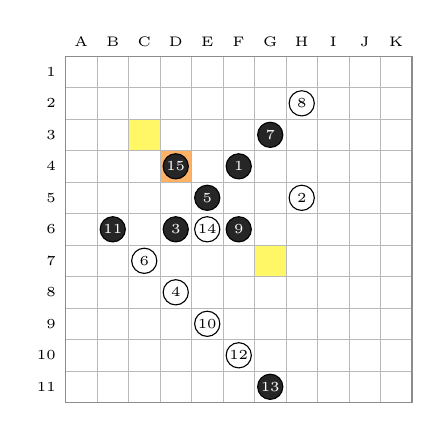
\begin{tikzpicture}[x=0.4cm, y=0.4cm]
\fill[orange!60] (3,-3) rectangle (4,-4);
\fill[yellow!60] (2,-2) rectangle (3,-3);
\fill[yellow!60] (6,-6) rectangle (7,-7);
\draw[gray!55, line width=.3pt, step=1] (0,0) grid (11,-11);
\draw[gray!90] (0,0) rectangle (11,-11);
\node[font=\tiny, anchor=south] at (0.5,0) {A};
\node[font=\tiny, anchor=south] at (1.5,0) {B};
\node[font=\tiny, anchor=south] at (2.5,0) {C};
\node[font=\tiny, anchor=south] at (3.5,0) {D};
\node[font=\tiny, anchor=south] at (4.5,0) {E};
\node[font=\tiny, anchor=south] at (5.5,0) {F};
\node[font=\tiny, anchor=south] at (6.5,0) {G};
\node[font=\tiny, anchor=south] at (7.5,0) {H};
\node[font=\tiny, anchor=south] at (8.5,0) {I};
\node[font=\tiny, anchor=south] at (9.5,0) {J};
\node[font=\tiny, anchor=south] at (10.5,0) {K};
\node[font=\tiny, anchor=east] at (0,-0.5) {1};
\node[font=\tiny, anchor=east] at (0,-1.5) {2};
\node[font=\tiny, anchor=east] at (0,-2.5) {3};
\node[font=\tiny, anchor=east] at (0,-3.5) {4};
\node[font=\tiny, anchor=east] at (0,-4.5) {5};
\node[font=\tiny, anchor=east] at (0,-5.5) {6};
\node[font=\tiny, anchor=east] at (0,-6.5) {7};
\node[font=\tiny, anchor=east] at (0,-7.5) {8};
\node[font=\tiny, anchor=east] at (0,-8.5) {9};
\node[font=\tiny, anchor=east] at (0,-9.5) {10};
\node[font=\tiny, anchor=east] at (0,-10.5) {11};
\draw[fill=white, line width=.4pt] (7.5,-1.5) circle (.40);
\node[font=\tiny, text=black, inner sep=0pt] at (7.5,-1.5) {8};
\draw[fill=black!85, line width=.4pt] (6.5,-2.5) circle (.40);
\node[font=\tiny, text=white, inner sep=0pt] at (6.5,-2.5) {7};
\draw[fill=black!85, line width=.4pt] (3.5,-3.5) circle (.40);
\node[font=\tiny, text=white, inner sep=0pt] at (3.5,-3.5) {15};
\draw[fill=black!85, line width=.4pt] (5.5,-3.5) circle (.40);
\node[font=\tiny, text=white, inner sep=0pt] at (5.5,-3.5) {1};
\draw[fill=black!85, line width=.4pt] (4.5,-4.5) circle (.40);
\node[font=\tiny, text=white, inner sep=0pt] at (4.5,-4.5) {5};
\draw[fill=white, line width=.4pt] (7.5,-4.5) circle (.40);
\node[font=\tiny, text=black, inner sep=0pt] at (7.5,-4.5) {2};
\draw[fill=black!85, line width=.4pt] (1.5,-5.5) circle (.40);
\node[font=\tiny, text=white, inner sep=0pt] at (1.5,-5.5) {11};
\draw[fill=black!85, line width=.4pt] (3.5,-5.5) circle (.40);
\node[font=\tiny, text=white, inner sep=0pt] at (3.5,-5.5) {3};
\draw[fill=white, line width=.4pt] (4.5,-5.5) circle (.40);
\node[font=\tiny, text=black, inner sep=0pt] at (4.5,-5.5) {14};
\draw[fill=black!85, line width=.4pt] (5.5,-5.5) circle (.40);
\node[font=\tiny, text=white, inner sep=0pt] at (5.5,-5.5) {9};
\draw[fill=white, line width=.4pt] (2.5,-6.5) circle (.40);
\node[font=\tiny, text=black, inner sep=0pt] at (2.5,-6.5) {6};
\draw[fill=white, line width=.4pt] (3.5,-7.5) circle (.40);
\node[font=\tiny, text=black, inner sep=0pt] at (3.5,-7.5) {4};
\draw[fill=white, line width=.4pt] (4.5,-8.5) circle (.40);
\node[font=\tiny, text=black, inner sep=0pt] at (4.5,-8.5) {10};
\draw[fill=white, line width=.4pt] (5.5,-9.5) circle (.40);
\node[font=\tiny, text=black, inner sep=0pt] at (5.5,-9.5) {12};
\draw[fill=black!85, line width=.4pt] (6.5,-10.5) circle (.40);
\node[font=\tiny, text=white, inner sep=0pt] at (6.5,-10.5) {13};
\end{tikzpicture}
    \caption{Sau nước 15 (ô cam); ô vàng là điểm đe doạ nó tạo ra}
  \end{subfigure}
  \par\medskip
  \begin{subfigure}[t]{.48\linewidth}
    \centering
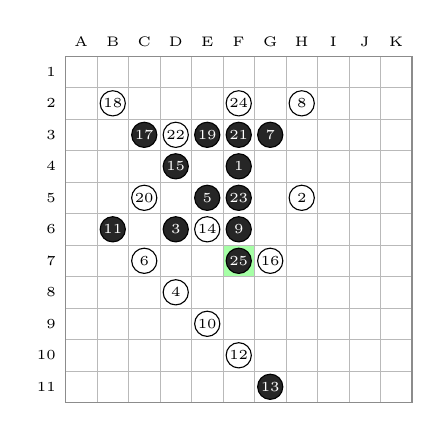
\begin{tikzpicture}[x=0.4cm, y=0.4cm]
\fill[green!35] (5,-6) rectangle (6,-7);
\draw[gray!55, line width=.3pt, step=1] (0,0) grid (11,-11);
\draw[gray!90] (0,0) rectangle (11,-11);
\node[font=\tiny, anchor=south] at (0.5,0) {A};
\node[font=\tiny, anchor=south] at (1.5,0) {B};
\node[font=\tiny, anchor=south] at (2.5,0) {C};
\node[font=\tiny, anchor=south] at (3.5,0) {D};
\node[font=\tiny, anchor=south] at (4.5,0) {E};
\node[font=\tiny, anchor=south] at (5.5,0) {F};
\node[font=\tiny, anchor=south] at (6.5,0) {G};
\node[font=\tiny, anchor=south] at (7.5,0) {H};
\node[font=\tiny, anchor=south] at (8.5,0) {I};
\node[font=\tiny, anchor=south] at (9.5,0) {J};
\node[font=\tiny, anchor=south] at (10.5,0) {K};
\node[font=\tiny, anchor=east] at (0,-0.5) {1};
\node[font=\tiny, anchor=east] at (0,-1.5) {2};
\node[font=\tiny, anchor=east] at (0,-2.5) {3};
\node[font=\tiny, anchor=east] at (0,-3.5) {4};
\node[font=\tiny, anchor=east] at (0,-4.5) {5};
\node[font=\tiny, anchor=east] at (0,-5.5) {6};
\node[font=\tiny, anchor=east] at (0,-6.5) {7};
\node[font=\tiny, anchor=east] at (0,-7.5) {8};
\node[font=\tiny, anchor=east] at (0,-8.5) {9};
\node[font=\tiny, anchor=east] at (0,-9.5) {10};
\node[font=\tiny, anchor=east] at (0,-10.5) {11};
\draw[fill=white, line width=.4pt] (1.5,-1.5) circle (.40);
\node[font=\tiny, text=black, inner sep=0pt] at (1.5,-1.5) {18};
\draw[fill=white, line width=.4pt] (5.5,-1.5) circle (.40);
\node[font=\tiny, text=black, inner sep=0pt] at (5.5,-1.5) {24};
\draw[fill=white, line width=.4pt] (7.5,-1.5) circle (.40);
\node[font=\tiny, text=black, inner sep=0pt] at (7.5,-1.5) {8};
\draw[fill=black!85, line width=.4pt] (2.5,-2.5) circle (.40);
\node[font=\tiny, text=white, inner sep=0pt] at (2.5,-2.5) {17};
\draw[fill=white, line width=.4pt] (3.5,-2.5) circle (.40);
\node[font=\tiny, text=black, inner sep=0pt] at (3.5,-2.5) {22};
\draw[fill=black!85, line width=.4pt] (4.5,-2.5) circle (.40);
\node[font=\tiny, text=white, inner sep=0pt] at (4.5,-2.5) {19};
\draw[fill=black!85, line width=.4pt] (5.5,-2.5) circle (.40);
\node[font=\tiny, text=white, inner sep=0pt] at (5.5,-2.5) {21};
\draw[fill=black!85, line width=.4pt] (6.5,-2.5) circle (.40);
\node[font=\tiny, text=white, inner sep=0pt] at (6.5,-2.5) {7};
\draw[fill=black!85, line width=.4pt] (3.5,-3.5) circle (.40);
\node[font=\tiny, text=white, inner sep=0pt] at (3.5,-3.5) {15};
\draw[fill=black!85, line width=.4pt] (5.5,-3.5) circle (.40);
\node[font=\tiny, text=white, inner sep=0pt] at (5.5,-3.5) {1};
\draw[fill=white, line width=.4pt] (2.5,-4.5) circle (.40);
\node[font=\tiny, text=black, inner sep=0pt] at (2.5,-4.5) {20};
\draw[fill=black!85, line width=.4pt] (4.5,-4.5) circle (.40);
\node[font=\tiny, text=white, inner sep=0pt] at (4.5,-4.5) {5};
\draw[fill=black!85, line width=.4pt] (5.5,-4.5) circle (.40);
\node[font=\tiny, text=white, inner sep=0pt] at (5.5,-4.5) {23};
\draw[fill=white, line width=.4pt] (7.5,-4.5) circle (.40);
\node[font=\tiny, text=black, inner sep=0pt] at (7.5,-4.5) {2};
\draw[fill=black!85, line width=.4pt] (1.5,-5.5) circle (.40);
\node[font=\tiny, text=white, inner sep=0pt] at (1.5,-5.5) {11};
\draw[fill=black!85, line width=.4pt] (3.5,-5.5) circle (.40);
\node[font=\tiny, text=white, inner sep=0pt] at (3.5,-5.5) {3};
\draw[fill=white, line width=.4pt] (4.5,-5.5) circle (.40);
\node[font=\tiny, text=black, inner sep=0pt] at (4.5,-5.5) {14};
\draw[fill=black!85, line width=.4pt] (5.5,-5.5) circle (.40);
\node[font=\tiny, text=white, inner sep=0pt] at (5.5,-5.5) {9};
\draw[fill=white, line width=.4pt] (2.5,-6.5) circle (.40);
\node[font=\tiny, text=black, inner sep=0pt] at (2.5,-6.5) {6};
\draw[fill=black!85, line width=.4pt] (5.5,-6.5) circle (.40);
\node[font=\tiny, text=white, inner sep=0pt] at (5.5,-6.5) {25};
\draw[fill=white, line width=.4pt] (6.5,-6.5) circle (.40);
\node[font=\tiny, text=black, inner sep=0pt] at (6.5,-6.5) {16};
\draw[fill=white, line width=.4pt] (3.5,-7.5) circle (.40);
\node[font=\tiny, text=black, inner sep=0pt] at (3.5,-7.5) {4};
\draw[fill=white, line width=.4pt] (4.5,-8.5) circle (.40);
\node[font=\tiny, text=black, inner sep=0pt] at (4.5,-8.5) {10};
\draw[fill=white, line width=.4pt] (5.5,-9.5) circle (.40);
\node[font=\tiny, text=black, inner sep=0pt] at (5.5,-9.5) {12};
\draw[fill=black!85, line width=.4pt] (6.5,-10.5) circle (.40);
\node[font=\tiny, text=white, inner sep=0pt] at (6.5,-10.5) {13};
\end{tikzpicture}
    \caption{Thế cuối (ô xanh: nước kết thúc)}
  \end{subfigure}
  \par\medskip
  \caption{Ván 1202: X là L2, O là L8, L2 thắng. Số trên quân là thứ tự nước.}
  \label{fig:cs-vs-1202}
\end{figure}

\paragraph{Diễn biến.} L2 dựng đe doạ sớm: E5 (ba hở chéo ngược, nước 5), G3 (tứ chéo ngược, nước 7). L8 đỡ và ở nước 10
(E9) còn tạo được một ba hở.

\paragraph{Nước 14 và nước khoá ván 15.} E6 là một nước yên tĩnh: không chặn gì, cũng không tạo đe doạ. Sau nó, bộ giải
chứng minh X thắng ép từ nước 15, với nước mở đầu F5 và hai đáp trả F3, F7 của O đều bị bác bỏ. Bốn ô H1, H3, H4, H6
tránh được chuỗi đó ở độ sâu của bộ giải. Tìm sâu hơn bác bỏ H1 và H6; với H3 và H4 bộ giải không tìm thấy đường thắng,
nhưng KataGomo chấm O khoảng $0\%$. Không đủ cơ sở để nói một nước khác ở lượt 14 đã cứu được ván.

\paragraph{Vì sao L2 thắng.} L2 không đi đúng nước mở đầu mà bộ giải tìm ra (nó đi D4, tạo ba hở chéo xuôi), nhưng vẫn
giữ được đường thắng ép ở mọi lượt sau. Từ nước 15, cả sáu nước của X đều là đe doạ, L8 chỉ còn đỡ. Nước 21 (F3) tạo
cùng lúc tứ ngang và ba hở dọc; nước 23 (F5) tạo tứ hở dọc với hai ô thắng F2 và F7. L8 chỉ chặn được F2, X kết thúc tại
F7. Một tác tử luật nhìn một nước đủ để thắng khi thế đã nghiêng: nó chỉ cần liên tục tạo đe doạ mà đối thủ buộc đỡ.
\par{\scriptsize
\renewcommand{\arraystretch}{0.95}
\begin{longtable}{rlp{4.4cm}lrll}
  \caption{Diễn biến ván 1202 sau khai cuộc}\label{tab:cs-vs-1202}\\
    \toprule
    Nước & Đi & Hình tạo / đỡ & Thắng ép & X \% & KG &  \\
    \midrule
  \endfirsthead
    \toprule
    Nước & Đi & Hình tạo / đỡ & Thắng ép & X \% & KG &  \\
    \midrule
  \endhead
    \bottomrule
  \endfoot
    5 & X E5 & ba hở chéo ngược & --- & 95 & D3 &  \\
    6 & O C7 & chặn đòn kép & --- & 98 & C7 &  \\
    7 & X G3 & tứ chéo ngược & --- & 97 & H4 &  \\
    8 & O H2 & chặn năm & --- & 94 & H2 &  \\
    9 & X F6 & --- & --- & 95 & F6 &  \\
    10 & O E9 & ba hở chéo xuôi & --- & 98 & H4 &  \\
    11 & X B6 & chặn đòn kép & --- & 99 & B6 &  \\
    12 & O F10 & tứ chéo xuôi & --- & 100 & D4 &  \\
    13 & X G11 & chặn năm & --- & 99 & G11 &  \\
    14 & O E6 & --- & --- & 99 & C8 &  \\
    15 & X D4 & ba hở chéo xuôi & VCT (F5) & 99 & E3 & \textbf{khoá ván} \\
    16 & O G7 & chặn đòn kép & --- & 100 & C3 &  \\
    17 & X C3 & tứ chéo xuôi & VCT (D3) & 100 & C3 &  \\
    18 & O B2 & chặn năm & --- & 100 & B2 &  \\
    19 & X E3 & ba hở chéo ngược & VCT (D3) & 100 & D3 &  \\
    20 & O C5 & chặn đòn kép & --- & 100 & F2 &  \\
    21 & X F3 & tứ ngang, ba hở dọc & VCF (D3) & 100 & F3 &  \\
    22 & O D3 & chặn năm & --- & 100 & D3 &  \\
    23 & X F5 & tứ hở dọc & VCF (F5) & 100 & F5 &  \\
    24 & O F2 & chặn năm & --- & 100 & F2 &  \\
    25 & X F7 & năm dọc & VCF (F7) & 100 & F7 &  \\
\end{longtable}
}


\subsection{Ván 2726: L7 thắng L8 bằng một chuỗi tứ dài}
\label{sec:cs-vs-2726}
L7 cầm X, L8 cầm O, khai cuộc H7--E4--F7--E5. KataGomo chấm X $97\%$ trước nước 5; điểm của O không vượt quá $8\%$ sau đó.
\begin{figure}[!htbp]
  \centering
  \begin{subfigure}[t]{.48\linewidth}
    \centering
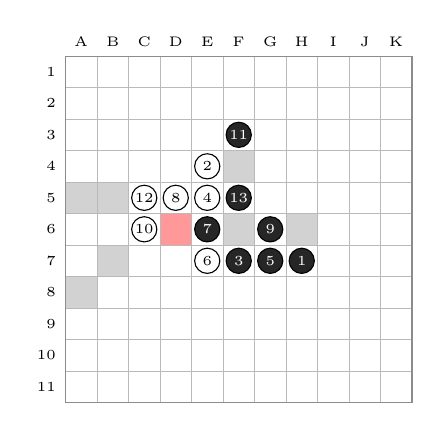
\begin{tikzpicture}[x=0.4cm, y=0.4cm]
\fill[gray!35] (5,-3) rectangle (6,-4);
\fill[gray!35] (0,-4) rectangle (1,-5);
\fill[gray!35] (1,-4) rectangle (2,-5);
\fill[gray!35] (5,-5) rectangle (6,-6);
\fill[gray!35] (7,-5) rectangle (8,-6);
\fill[gray!35] (1,-6) rectangle (2,-7);
\fill[gray!35] (0,-7) rectangle (1,-8);
\fill[red!40] (3,-5) rectangle (4,-6);
\draw[gray!55, line width=.3pt, step=1] (0,0) grid (11,-11);
\draw[gray!90] (0,0) rectangle (11,-11);
\node[font=\tiny, anchor=south] at (0.5,0) {A};
\node[font=\tiny, anchor=south] at (1.5,0) {B};
\node[font=\tiny, anchor=south] at (2.5,0) {C};
\node[font=\tiny, anchor=south] at (3.5,0) {D};
\node[font=\tiny, anchor=south] at (4.5,0) {E};
\node[font=\tiny, anchor=south] at (5.5,0) {F};
\node[font=\tiny, anchor=south] at (6.5,0) {G};
\node[font=\tiny, anchor=south] at (7.5,0) {H};
\node[font=\tiny, anchor=south] at (8.5,0) {I};
\node[font=\tiny, anchor=south] at (9.5,0) {J};
\node[font=\tiny, anchor=south] at (10.5,0) {K};
\node[font=\tiny, anchor=east] at (0,-0.5) {1};
\node[font=\tiny, anchor=east] at (0,-1.5) {2};
\node[font=\tiny, anchor=east] at (0,-2.5) {3};
\node[font=\tiny, anchor=east] at (0,-3.5) {4};
\node[font=\tiny, anchor=east] at (0,-4.5) {5};
\node[font=\tiny, anchor=east] at (0,-5.5) {6};
\node[font=\tiny, anchor=east] at (0,-6.5) {7};
\node[font=\tiny, anchor=east] at (0,-7.5) {8};
\node[font=\tiny, anchor=east] at (0,-8.5) {9};
\node[font=\tiny, anchor=east] at (0,-9.5) {10};
\node[font=\tiny, anchor=east] at (0,-10.5) {11};
\draw[fill=black!85, line width=.4pt] (5.5,-2.5) circle (.40);
\node[font=\tiny, text=white, inner sep=0pt] at (5.5,-2.5) {11};
\draw[fill=white, line width=.4pt] (4.5,-3.5) circle (.40);
\node[font=\tiny, text=black, inner sep=0pt] at (4.5,-3.5) {2};
\draw[fill=white, line width=.4pt] (2.5,-4.5) circle (.40);
\node[font=\tiny, text=black, inner sep=0pt] at (2.5,-4.5) {12};
\draw[fill=white, line width=.4pt] (3.5,-4.5) circle (.40);
\node[font=\tiny, text=black, inner sep=0pt] at (3.5,-4.5) {8};
\draw[fill=white, line width=.4pt] (4.5,-4.5) circle (.40);
\node[font=\tiny, text=black, inner sep=0pt] at (4.5,-4.5) {4};
\draw[fill=black!85, line width=.4pt] (5.5,-4.5) circle (.40);
\node[font=\tiny, text=white, inner sep=0pt] at (5.5,-4.5) {13};
\draw[fill=white, line width=.4pt] (2.5,-5.5) circle (.40);
\node[font=\tiny, text=black, inner sep=0pt] at (2.5,-5.5) {10};
\draw[fill=black!85, line width=.4pt] (4.5,-5.5) circle (.40);
\node[font=\tiny, text=white, inner sep=0pt] at (4.5,-5.5) {7};
\draw[fill=black!85, line width=.4pt] (6.5,-5.5) circle (.40);
\node[font=\tiny, text=white, inner sep=0pt] at (6.5,-5.5) {9};
\draw[fill=white, line width=.4pt] (4.5,-6.5) circle (.40);
\node[font=\tiny, text=black, inner sep=0pt] at (4.5,-6.5) {6};
\draw[fill=black!85, line width=.4pt] (5.5,-6.5) circle (.40);
\node[font=\tiny, text=white, inner sep=0pt] at (5.5,-6.5) {3};
\draw[fill=black!85, line width=.4pt] (6.5,-6.5) circle (.40);
\node[font=\tiny, text=white, inner sep=0pt] at (6.5,-6.5) {5};
\draw[fill=black!85, line width=.4pt] (7.5,-6.5) circle (.40);
\node[font=\tiny, text=white, inner sep=0pt] at (7.5,-6.5) {1};
\end{tikzpicture}
    \caption{Trước nước 14: ô đỏ là nước đã đi; 7 ô xám chỉ hoãn thua, không cứu được}
  \end{subfigure}
  \hfill
  \begin{subfigure}[t]{.48\linewidth}
    \centering
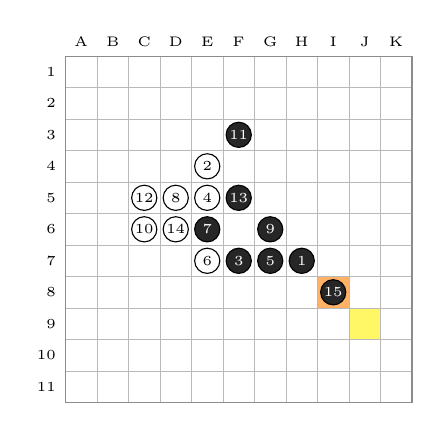
\begin{tikzpicture}[x=0.4cm, y=0.4cm]
\fill[orange!60] (8,-7) rectangle (9,-8);
\fill[yellow!60] (9,-8) rectangle (10,-9);
\draw[gray!55, line width=.3pt, step=1] (0,0) grid (11,-11);
\draw[gray!90] (0,0) rectangle (11,-11);
\node[font=\tiny, anchor=south] at (0.5,0) {A};
\node[font=\tiny, anchor=south] at (1.5,0) {B};
\node[font=\tiny, anchor=south] at (2.5,0) {C};
\node[font=\tiny, anchor=south] at (3.5,0) {D};
\node[font=\tiny, anchor=south] at (4.5,0) {E};
\node[font=\tiny, anchor=south] at (5.5,0) {F};
\node[font=\tiny, anchor=south] at (6.5,0) {G};
\node[font=\tiny, anchor=south] at (7.5,0) {H};
\node[font=\tiny, anchor=south] at (8.5,0) {I};
\node[font=\tiny, anchor=south] at (9.5,0) {J};
\node[font=\tiny, anchor=south] at (10.5,0) {K};
\node[font=\tiny, anchor=east] at (0,-0.5) {1};
\node[font=\tiny, anchor=east] at (0,-1.5) {2};
\node[font=\tiny, anchor=east] at (0,-2.5) {3};
\node[font=\tiny, anchor=east] at (0,-3.5) {4};
\node[font=\tiny, anchor=east] at (0,-4.5) {5};
\node[font=\tiny, anchor=east] at (0,-5.5) {6};
\node[font=\tiny, anchor=east] at (0,-6.5) {7};
\node[font=\tiny, anchor=east] at (0,-7.5) {8};
\node[font=\tiny, anchor=east] at (0,-8.5) {9};
\node[font=\tiny, anchor=east] at (0,-9.5) {10};
\node[font=\tiny, anchor=east] at (0,-10.5) {11};
\draw[fill=black!85, line width=.4pt] (5.5,-2.5) circle (.40);
\node[font=\tiny, text=white, inner sep=0pt] at (5.5,-2.5) {11};
\draw[fill=white, line width=.4pt] (4.5,-3.5) circle (.40);
\node[font=\tiny, text=black, inner sep=0pt] at (4.5,-3.5) {2};
\draw[fill=white, line width=.4pt] (2.5,-4.5) circle (.40);
\node[font=\tiny, text=black, inner sep=0pt] at (2.5,-4.5) {12};
\draw[fill=white, line width=.4pt] (3.5,-4.5) circle (.40);
\node[font=\tiny, text=black, inner sep=0pt] at (3.5,-4.5) {8};
\draw[fill=white, line width=.4pt] (4.5,-4.5) circle (.40);
\node[font=\tiny, text=black, inner sep=0pt] at (4.5,-4.5) {4};
\draw[fill=black!85, line width=.4pt] (5.5,-4.5) circle (.40);
\node[font=\tiny, text=white, inner sep=0pt] at (5.5,-4.5) {13};
\draw[fill=white, line width=.4pt] (2.5,-5.5) circle (.40);
\node[font=\tiny, text=black, inner sep=0pt] at (2.5,-5.5) {10};
\draw[fill=white, line width=.4pt] (3.5,-5.5) circle (.40);
\node[font=\tiny, text=black, inner sep=0pt] at (3.5,-5.5) {14};
\draw[fill=black!85, line width=.4pt] (4.5,-5.5) circle (.40);
\node[font=\tiny, text=white, inner sep=0pt] at (4.5,-5.5) {7};
\draw[fill=black!85, line width=.4pt] (6.5,-5.5) circle (.40);
\node[font=\tiny, text=white, inner sep=0pt] at (6.5,-5.5) {9};
\draw[fill=white, line width=.4pt] (4.5,-6.5) circle (.40);
\node[font=\tiny, text=black, inner sep=0pt] at (4.5,-6.5) {6};
\draw[fill=black!85, line width=.4pt] (5.5,-6.5) circle (.40);
\node[font=\tiny, text=white, inner sep=0pt] at (5.5,-6.5) {3};
\draw[fill=black!85, line width=.4pt] (6.5,-6.5) circle (.40);
\node[font=\tiny, text=white, inner sep=0pt] at (6.5,-6.5) {5};
\draw[fill=black!85, line width=.4pt] (7.5,-6.5) circle (.40);
\node[font=\tiny, text=white, inner sep=0pt] at (7.5,-6.5) {1};
\draw[fill=black!85, line width=.4pt] (8.5,-7.5) circle (.40);
\node[font=\tiny, text=white, inner sep=0pt] at (8.5,-7.5) {15};
\end{tikzpicture}
    \caption{Sau nước 15 (ô cam); ô vàng là điểm đe doạ nó tạo ra}
  \end{subfigure}
  \par\medskip
  \begin{subfigure}[t]{.48\linewidth}
    \centering
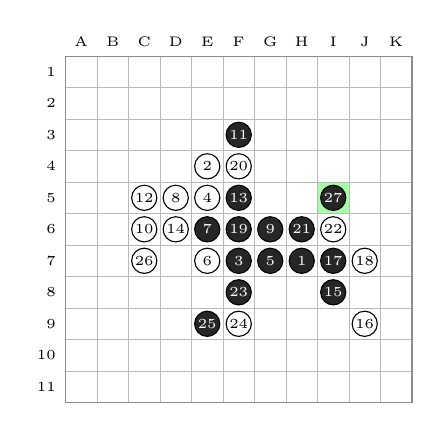
\begin{tikzpicture}[x=0.4cm, y=0.4cm]
\fill[green!35] (8,-4) rectangle (9,-5);
\draw[gray!55, line width=.3pt, step=1] (0,0) grid (11,-11);
\draw[gray!90] (0,0) rectangle (11,-11);
\node[font=\tiny, anchor=south] at (0.5,0) {A};
\node[font=\tiny, anchor=south] at (1.5,0) {B};
\node[font=\tiny, anchor=south] at (2.5,0) {C};
\node[font=\tiny, anchor=south] at (3.5,0) {D};
\node[font=\tiny, anchor=south] at (4.5,0) {E};
\node[font=\tiny, anchor=south] at (5.5,0) {F};
\node[font=\tiny, anchor=south] at (6.5,0) {G};
\node[font=\tiny, anchor=south] at (7.5,0) {H};
\node[font=\tiny, anchor=south] at (8.5,0) {I};
\node[font=\tiny, anchor=south] at (9.5,0) {J};
\node[font=\tiny, anchor=south] at (10.5,0) {K};
\node[font=\tiny, anchor=east] at (0,-0.5) {1};
\node[font=\tiny, anchor=east] at (0,-1.5) {2};
\node[font=\tiny, anchor=east] at (0,-2.5) {3};
\node[font=\tiny, anchor=east] at (0,-3.5) {4};
\node[font=\tiny, anchor=east] at (0,-4.5) {5};
\node[font=\tiny, anchor=east] at (0,-5.5) {6};
\node[font=\tiny, anchor=east] at (0,-6.5) {7};
\node[font=\tiny, anchor=east] at (0,-7.5) {8};
\node[font=\tiny, anchor=east] at (0,-8.5) {9};
\node[font=\tiny, anchor=east] at (0,-9.5) {10};
\node[font=\tiny, anchor=east] at (0,-10.5) {11};
\draw[fill=black!85, line width=.4pt] (5.5,-2.5) circle (.40);
\node[font=\tiny, text=white, inner sep=0pt] at (5.5,-2.5) {11};
\draw[fill=white, line width=.4pt] (4.5,-3.5) circle (.40);
\node[font=\tiny, text=black, inner sep=0pt] at (4.5,-3.5) {2};
\draw[fill=white, line width=.4pt] (5.5,-3.5) circle (.40);
\node[font=\tiny, text=black, inner sep=0pt] at (5.5,-3.5) {20};
\draw[fill=white, line width=.4pt] (2.5,-4.5) circle (.40);
\node[font=\tiny, text=black, inner sep=0pt] at (2.5,-4.5) {12};
\draw[fill=white, line width=.4pt] (3.5,-4.5) circle (.40);
\node[font=\tiny, text=black, inner sep=0pt] at (3.5,-4.5) {8};
\draw[fill=white, line width=.4pt] (4.5,-4.5) circle (.40);
\node[font=\tiny, text=black, inner sep=0pt] at (4.5,-4.5) {4};
\draw[fill=black!85, line width=.4pt] (5.5,-4.5) circle (.40);
\node[font=\tiny, text=white, inner sep=0pt] at (5.5,-4.5) {13};
\draw[fill=black!85, line width=.4pt] (8.5,-4.5) circle (.40);
\node[font=\tiny, text=white, inner sep=0pt] at (8.5,-4.5) {27};
\draw[fill=white, line width=.4pt] (2.5,-5.5) circle (.40);
\node[font=\tiny, text=black, inner sep=0pt] at (2.5,-5.5) {10};
\draw[fill=white, line width=.4pt] (3.5,-5.5) circle (.40);
\node[font=\tiny, text=black, inner sep=0pt] at (3.5,-5.5) {14};
\draw[fill=black!85, line width=.4pt] (4.5,-5.5) circle (.40);
\node[font=\tiny, text=white, inner sep=0pt] at (4.5,-5.5) {7};
\draw[fill=black!85, line width=.4pt] (5.5,-5.5) circle (.40);
\node[font=\tiny, text=white, inner sep=0pt] at (5.5,-5.5) {19};
\draw[fill=black!85, line width=.4pt] (6.5,-5.5) circle (.40);
\node[font=\tiny, text=white, inner sep=0pt] at (6.5,-5.5) {9};
\draw[fill=black!85, line width=.4pt] (7.5,-5.5) circle (.40);
\node[font=\tiny, text=white, inner sep=0pt] at (7.5,-5.5) {21};
\draw[fill=white, line width=.4pt] (8.5,-5.5) circle (.40);
\node[font=\tiny, text=black, inner sep=0pt] at (8.5,-5.5) {22};
\draw[fill=white, line width=.4pt] (2.5,-6.5) circle (.40);
\node[font=\tiny, text=black, inner sep=0pt] at (2.5,-6.5) {26};
\draw[fill=white, line width=.4pt] (4.5,-6.5) circle (.40);
\node[font=\tiny, text=black, inner sep=0pt] at (4.5,-6.5) {6};
\draw[fill=black!85, line width=.4pt] (5.5,-6.5) circle (.40);
\node[font=\tiny, text=white, inner sep=0pt] at (5.5,-6.5) {3};
\draw[fill=black!85, line width=.4pt] (6.5,-6.5) circle (.40);
\node[font=\tiny, text=white, inner sep=0pt] at (6.5,-6.5) {5};
\draw[fill=black!85, line width=.4pt] (7.5,-6.5) circle (.40);
\node[font=\tiny, text=white, inner sep=0pt] at (7.5,-6.5) {1};
\draw[fill=black!85, line width=.4pt] (8.5,-6.5) circle (.40);
\node[font=\tiny, text=white, inner sep=0pt] at (8.5,-6.5) {17};
\draw[fill=white, line width=.4pt] (9.5,-6.5) circle (.40);
\node[font=\tiny, text=black, inner sep=0pt] at (9.5,-6.5) {18};
\draw[fill=black!85, line width=.4pt] (5.5,-7.5) circle (.40);
\node[font=\tiny, text=white, inner sep=0pt] at (5.5,-7.5) {23};
\draw[fill=black!85, line width=.4pt] (8.5,-7.5) circle (.40);
\node[font=\tiny, text=white, inner sep=0pt] at (8.5,-7.5) {15};
\draw[fill=black!85, line width=.4pt] (4.5,-8.5) circle (.40);
\node[font=\tiny, text=white, inner sep=0pt] at (4.5,-8.5) {25};
\draw[fill=white, line width=.4pt] (5.5,-8.5) circle (.40);
\node[font=\tiny, text=black, inner sep=0pt] at (5.5,-8.5) {24};
\draw[fill=white, line width=.4pt] (9.5,-8.5) circle (.40);
\node[font=\tiny, text=black, inner sep=0pt] at (9.5,-8.5) {16};
\end{tikzpicture}
    \caption{Thế cuối (ô xanh: nước kết thúc)}
  \end{subfigure}
  \par\medskip
  \caption{Ván 2726: X là L7, O là L8, L7 thắng. Số trên quân là thứ tự nước.}
  \label{fig:cs-vs-2726}
\end{figure}

\paragraph{Diễn biến.} Hai bên đổi đe doạ: L7 tạo ba hở ngang ở nước 5, L8 đáp bằng ba hở ở nước 10 (C6) và nước 12 (C5).
L7 chặn cả hai (F3, F5), và điểm engine của X lên $100\%$.

\paragraph{Nước 14 và nước khoá ván 15.} L8 tiếp tục tấn công bằng một ba hở chéo xuôi (D6). Lúc đó X đã đủ quân cho chuỗi
tứ F6--F4--H6--I6--F8--F9--I5--J4--E9. Mỗi nước tứ buộc đối thủ đỡ ngay, nên ba hở của O không kịp phát huy: \emph{tứ
nhanh hơn ba}. Bảy ô (F4, A5, B5, F6, H6, B7, A8) tránh được chuỗi tứ này, nhưng cả bảy đều bị bác bỏ khi tìm sâu hơn một
bậc và engine chấm O $0\%$. D6 làm ván kết thúc nhanh hơn; thế đã thua từ trước.

\paragraph{Vì sao L7 thắng.} L7 không đi đường ngắn nhất ngay: nó chèn hai nước tứ khác (I8 ở nước 15, I7 ở nước 17) rồi
mới đi F6. Đường thắng vẫn được giữ qua mọi lượt. Nước 23 (F8) vừa chặn vừa tạo tứ dọc và ba hở; nước 25 (E9) tạo tứ hở
chéo ngược với hai ô thắng I5 và D10. L8 đi C7 để dựng tứ hở của mình, nhưng đến lượt X trước, và I5 kết thúc ván.
\par{\scriptsize
\renewcommand{\arraystretch}{0.95}
\begin{longtable}{rlp{4.4cm}lrll}
  \caption{Diễn biến ván 2726 sau khai cuộc}\label{tab:cs-vs-2726}\\
    \toprule
    Nước & Đi & Hình tạo / đỡ & Thắng ép & X \% & KG &  \\
    \midrule
  \endfirsthead
    \toprule
    Nước & Đi & Hình tạo / đỡ & Thắng ép & X \% & KG &  \\
    \midrule
  \endhead
    \bottomrule
  \endfoot
    5 & X G7 & ba hở ngang & --- & 97 & G8 &  \\
    6 & O E7 & chặn đòn kép, ba hở dọc & --- & 92 & E7 &  \\
    7 & X E6 & chặn đòn kép & --- & 94 & E6 &  \\
    8 & O D5 & --- & --- & 95 & C5 &  \\
    9 & X G6 & --- & --- & 95 & G6 &  \\
    10 & O C6 & ba hở chéo ngược & --- & 94 & C5 &  \\
    11 & X F3 & chặn đòn kép & --- & 99 & F3 &  \\
    12 & O C5 & ba hở ngang & --- & 99 & A8 &  \\
    13 & X F5 & chặn đòn kép & --- & 100 & F5 &  \\
    14 & O D6 & ba hở chéo xuôi & --- & 100 & F4 &  \\
    15 & X I8 & tứ chéo xuôi & VCF (F6) & 100 & F6 & \textbf{khoá ván} \\
    16 & O J9 & chặn năm & --- & 100 & J9 &  \\
    17 & X I7 & tứ ngang & VCF (F6) & 100 & F6 &  \\
    18 & O J7 & chặn năm & --- & 100 & J7 &  \\
    19 & X F6 & tứ dọc & VCF (F6) & 100 & F6 &  \\
    20 & O F4 & chặn năm, ba hở chéo ngược & --- & 100 & F4 &  \\
    21 & X H6 & tứ ngang & VCF (I6) & 100 & I6 &  \\
    22 & O I6 & chặn năm & --- & 100 & I6 &  \\
    23 & X F8 & chặn đòn kép, tứ dọc, ba hở chéo ngược & VCF (F8) & 100 & F8 &  \\
    24 & O F9 & chặn năm & --- & 100 & F9 &  \\
    25 & X E9 & tứ hở chéo ngược & VCF (I5) & 100 & I5 &  \\
    26 & O C7 & chặn đòn kép, ba hở dọc, tứ hở chéo ngược & --- & 100 & D10 &  \\
    27 & X I5 & chặn đòn kép, năm chéo ngược & VCF (I5) & 100 & D10 &  \\
\end{longtable}
}


\subsection{Các nước thay thế có cứu được ván không}
Bảng~\ref{tab:cs-vs-thay-the} gom kết quả kiểm mọi ô thay thế ở lượt ngay trước nước khoá ván. Chỉ ở ván 13 các ô đó
thật sự giữ được thế: cả ba không bị bác bỏ và được engine chấm $44$--$46\%$, bằng với đánh giá trước khi đi, trong khi
nước đã đi còn $0\%$. Ở ba ván kia, ``tránh được chuỗi ép ngắn'' không đồng nghĩa với ``cứu được ván''. Đây cũng là lời
nhắc về mọi số đo dựa trên bộ giải có độ sâu giới hạn.
\begin{table}[H]
  \centering
  \footnotesize
  \caption{Các nước thay thế cho sai lầm quyết định của bốn ván}
  \label{tab:cs-vs-thay-the}
  \begin{tabular}{rlllr}
    \toprule
    Ván & Nước & Ô & Tìm sâu hơn một bậc (3 đe doạ) & KG \% \\
    \midrule
    13 & 31 (X) & B6 (đã đi) & bị thắng ép & 0 \\
     &  & H3 & không tìm thấy đường thắng ép & 45 \\
     &  & H4 & không tìm thấy đường thắng ép & 44 \\
     &  & C6 & không tìm thấy đường thắng ép & 46 \\
    \midrule
    26 & 16 (O) & I5 (đã đi) & bị thắng ép & 0 \\
     &  & C8 & vẫn bị thắng ép, mở đầu D8 & 0 \\
    \midrule
    1202 & 14 (O) & E6 (đã đi) & bị thắng ép & 1 \\
     &  & H1 & vẫn bị thắng ép, mở đầu E6 & 0 \\
     &  & H3 & không tìm thấy đường thắng ép & 0 \\
     &  & H4 & không tìm thấy đường thắng ép & 0 \\
     &  & H6 & vẫn bị thắng ép, mở đầu F3 & 1 \\
    \midrule
    2726 & 14 (O) & D6 (đã đi) & bị thắng ép & 0 \\
     &  & F4 & vẫn bị thắng ép, mở đầu G4 & 0 \\
     &  & A5 & vẫn bị thắng ép, mở đầu B5 & 0 \\
     &  & B5 & vẫn bị thắng ép, mở đầu A5 & 0 \\
     &  & F6 & vẫn bị thắng ép, mở đầu G4 & 0 \\
     &  & H6 & vẫn bị thắng ép, mở đầu G4 & 0 \\
     &  & B7 & vẫn bị thắng ép, mở đầu A8 & 0 \\
     &  & A8 & vẫn bị thắng ép, mở đầu B7 & 0 \\
    \bottomrule
  \end{tabular}
  \par\smallskip\parbox{.95\linewidth}{\footnotesize ``KG'' là điểm KataGomo của bên vừa đi sau khi chọn ô đó (1\,600 lượt thăm).}
\end{table}


\subsection{Điểm chung của bốn ván}
\label{sec:cs-vs-chung}
\begin{enumerate}
  \item \textbf{Khai cuộc lệch về bên đi trước.} Trước nước đầu tiên của tác tử, KataGomo đã chấm X từ $82\%$ đến $97\%$ ở
  cả bốn khai cuộc. Ở ba ván 26, 1202 và 2726, bên cầm O thua khi chưa từng có thế cân bằng. Giải đấu đổi màu trên cùng
  khai cuộc để bù, nhưng kết quả của một ván riêng lẻ phụ thuộc mạnh vào màu quân, và nhiều cặp ván có thể chỉ đo bên nào
  được cầm X.
  \item \textbf{Mất quyền chủ động là mất ván.} Từ nước khoá ván, bên thắng liên tục ra đe doạ; nước của bên thua là nước
  chặn hoặc phản đòn đến chậm một lượt.
  \item \textbf{Sai lầm quyết định thật sự chỉ thấy ở ván 13:} một nước tứ mà ô chặn bắt buộc lại cho đối thủ một tứ. Cả
  hai bên trong ván này còn mất lợi thế nhiều lần (nước 9, 16, 25 theo engine) mà không có trọng tài nào ngoài engine
  nhận ra, cho thấy lỗi nhìn xa vẫn phổ biến ở hai tác tử mạnh nhất.
\end{enumerate}

\paragraph{Giới hạn.} Bốn ván là minh hoạ, không phải mẫu thống kê. Điểm của KataGomo là ước lượng của một mô hình huấn
luyện trên bàn 15$\times$15; riêng nhận định về khai cuộc cần được kiểm trên toàn bộ khai cuộc trước khi coi là kết luận.
